\begin{refsection}

% Variables
\newcommand{\baCovLayerDivB}{$\beta{}$=0.03$\pm$0.0076, F(2,167)=18, p<0.001, R\textsuperscript{2}=0.1}
\newcommand{\baCovFoliageB}{$\beta{}$=87$\pm$30, F(2,167)=8.6, p<0.01, R\textsuperscript{2}=0.05}
\newcommand{\baCovCoverB}{$\beta{}$=0.001$\pm$0.00048, F(2,168)=6.3, p<0.05, R\textsuperscript{2}=0.04}
\newcommand{\shannonLayerDivB}{$\beta{}$=1$\pm$0.27, F(2,180)=17, p<0.001, R\textsuperscript{2}=0.09}
\newcommand{\shannonFoliageB}{$\beta{}$=3163$\pm$1063, F(2,180)=8.9, p<0.01, R\textsuperscript{2}=0.05}
\newcommand{\shannonCoverB}{$\beta{}$=0.05$\pm$0.017, F(2,181)=7.3, p<0.01, R\textsuperscript{2}=0.04}
\newcommand{\winkelCoverPB}{$\beta{}$=-3$\pm$1.7, F(2,20)=3.9, p=0.06, R\textsuperscript{2}=0.2}
\newcommand{\voronoiCoverPB}{$\beta{}$=0.002$\pm$0.0058, F(2,20)=0.17, p=0.69, R\textsuperscript{2}=0.008}
\newcommand{\baCovCoverPB}{$\beta{}$=8e-04$\pm$0.00057, F(2,20)=2.2, p=0.15, R\textsuperscript{2}=0.1}
\newcommand{\baCovRoughPB}{$\beta{}$=0.03$\pm$0.05, F(2,16)=0.36, p=0.56, R\textsuperscript{2}=0.02}
\newcommand{\baCovRugosityPB}{$\beta{}$=-1$\pm$0.53, F(2,16)=3.7, p=0.07, R\textsuperscript{2}=0.2}
\newcommand{\shannonCoverPB}{$\beta{}$=0.01$\pm$0.012, F(2,20)=0.74, p=0.4, R\textsuperscript{2}=0.04}
\newcommand{\shannonHeightPB}{$\beta{}$=0.3$\pm$0.13, F(2,16)=6, p<0.05, R\textsuperscript{2}=0.3}
\newcommand{\shannonRoughPB}{$\beta{}$=-2$\pm$0.95, F(2,16)=4, p=0.06, R\textsuperscript{2}=0.2}
\newcommand{\shannonRugPB}{$\beta{}$=-13$\pm$12, F(2,16)=1.2, p=0.28, R\textsuperscript{2}=0.07}
\newcommand{\hemiCor}{$r$(195)=0.87, p<0.001}
\newcommand{\hemiLme}{$\beta$(173)=0.13$\pm$0.011, p=0.21}
\newcommand{\subModN}{4}
\newcommand{\bestLayerDivRsqS}{50}
\newcommand{\bestDensRsqS}{27}
\newcommand{\bestUnifRsqS}{29}
\newcommand{\bestCumRsqS}{29}
\newcommand{\shannonHeightP}{$\beta{}$=3$\pm$0.96, p<0.05}
\newcommand{\shannonCoverP}{$\beta{}$=0.07$\pm$0.085, p=0.41}
\newcommand{\shannonRoughP}{$\beta{}$=-13$\pm$6.8, p=0.09}
\newcommand{\shannonRugP}{$\beta{}$=-111$\pm$71, p=0.15}
\newcommand{\treeDensRugP}{$\beta{}$=-61$\pm$42, p=0.17}
\newcommand{\covBARoughP}{$\beta{}$=5$\pm$3.4, p=0.18}
\newcommand{\wiCoverP}{$\beta{}$=-0.08$\pm$0.043, p=0.1}
\newcommand{\baCoverP}{$\beta{}$=0.06$\pm$0.042, p=0.19}
\newcommand{\voronoiDensP}{$\beta{}$=6199$\pm$3312, p=0.09}
\newcommand{\shannonBaCoverPath}{-0.0016}
\newcommand{\shannonBaPath}{0.32***}
\newcommand{\hegyiBaPath}{0.16}
\newcommand{\baCoverPath}{-0.005}
\newcommand{\hegyiCoverPath}{0.7***}
\newcommand{\shannonCoverPath}{0.078}
\newcommand{\coverSemRm}{0.47}
\newcommand{\coverSemRc}{0.61}
\newcommand{\treeShannonBaPath}{0.57}
\newcommand{\treeShannonDensPath}{1.1*}
\newcommand{\treeShannonHeightPath}{1.3*}
\newcommand{\minglBaPath}{-0.47}
\newcommand{\minglDensPath}{-0.81}
\newcommand{\minglHeightPath}{-0.89}
\newcommand{\densHeightPath}{-0.027}
\newcommand{\baHeightPath}{0.037}
\newcommand{\heightSemRsq}{0.49}
\newcommand{\treeShannonBaHeightPath}{0.0210}
\newcommand{\treeShannonDensHeightPath}{-0.0294}
\newcommand{\perIndet}{0.2}
\newcommand{\rawpt}{2.9e+08}
\newcommand{\voxelpt}{4.5e+07}
\newcommand{\subpt}{2.1e+07}


\def\chaptertitle{TLS chapter}


\chapter[\chaptertitle]{\chaptertitle}
\chaptermark{Species diversity and canopy complexity}
\label{ch:tls}

The following chapter has been prepared for submission to \textit{Journal of Ecology}. Extended methods are presented in \autoref{ch:workflow}.

\paperauthors{John L. Godlee\textsuperscript{1}, Francisco Maiato Gon\c{c}alves\textsuperscript{2}, Jos\'{e} Jo\~{a}o Tchamba\textsuperscript{2}, Antonio Valter Chisingui\textsuperscript{2}, Casey M. Ryan\textsuperscript{1}, Kyle G. Dexter\textsuperscript{1,3}}

\begin{paperaffil}
\item{School of GeoSciences, University of Edinburgh, Edinburgh, EH9 3FF, United Kingdom}
\item{Herbarium of Lubango, ISCED Hu\'{i}la, Sarmento Rodrigues Str. No. 2, CP. 230, Lubango, Angola}
\item{Royal Botanic Garden Edinburgh, Edinburgh, EH3 5LR, United Kingdom}
\end{paperaffil}

\authorcontributions{JLG conceived the study, conducted the analysis, and wrote the first draft of the manuscript. KGD contributed to manuscript editing.}

\begin{abstract}
	Atmospheric CO\textsubscript{2} enrichment and human-induced climate change are expected to drive woody encroachment and increased tree growth rates across African savannas, with consequences for ecosystem function, particularly related to carbon dynamics. The vegetation dynamics of savanna-woodland mosaics are complex however, as woody growth is mediated by seasonal fire that is itself driven by properties of the woody overstorey. It is unclear how variation in tree species composition and stand structure in this ecosystem affects woody canopy complexity, and how this might determine future vegetation dynamics. Here, I conducted a study of canopy structure in southern African savannas using terrestrial LiDAR, at sites in Bicuar National Park, Angola and Mtarure Forest Reserve, Tanzania, to explore relationships between tree species diversity, species composition, the spatial distribution of trees, variation in tree size and canopy complexity. Species diversity was found to have consistent weak positive effects on plot scale canopy complexity metrics related to canopy density, but a negative effect on metrics related to the spatial heterogeneity of canopy material distribution. Species diversity was associated with an increase in canopy height, canopy closure, and within-canopy structural complexity, together suggesting that diverse canopies may promote woody encroachment and exhibit higher upper limits on biomass. Stochasticity in neighbourhood scale stand structure partially weakened species diversity effects at small spatial scales. Finally, while tree species diversity did affect tree size variation, tree size variation itself did not influence canopy complexity. As species diversity also influenced canopy foliage volume, this suggests a partial decoupling of tree stem size and canopy foliage volume, highlighting species-specific differences in crown shape that are independent from tree size.
\end{abstract}

\section{Introduction}
\label{tls:sec:intro}

% Woody encroachment and ecological change
Atmospheric CO\textsubscript{2} enrichment, coupled with climate change and changing disturbance regimes, is expected to drive woody encroachment, i.e. the proliferation of trees into previously non-wooded areas, along with increased stem density and growth of trees in currently wooded areas, here termed woody densification, across the savanna biome over the coming century \citep{Mitchard2013, Criado2020, Stevens2017}. As atmospheric CO\textsubscript{2} concentrations increase, C\textsubscript{3} trees are expected to gain a competitive edge over C\textsubscript{4} grasses due to differences in photosynthetic pathway and carbon use efficiency \citep{Buitenwerf2012}, allowing trees to increase their productivity. This is expected to have cascading effects on canopy cover, grass growth, and disturbance regime \citep{Bond2012}. If realised, woody encroachment and woody densification will have significant effects on the global carbon cycle, as more CO\textsubscript{2} is stored in woody biomass, as well as myriad other effects on ecosystem structure \citep{Donohue2013}. Indeed, tropical savannas have been identified as the fastest increasing component of the terrestrial carbon sink \citep{Sitch2015}. Previous studies however, have reported wide variation in rates of woody encroachment and densification \citep{Mitchard2013}, particularly in disturbance-prone savannas such as miombo woodlands in southern Africa \citep{Axelsson2018}, and it is unclear how the fertilisation effect of atmospheric CO\textsubscript{2} enrichment interacts with other ecosystem properties and processes to alter vegetation structure \citep{Korner2017, Reich2014}.

% Southern African woodlands 
Savanna vegetation is defined by the coexistence of trees and grasses \citep{Scholes1997}. In the tropical mesic savannas of southern Africa, disturbance by fire and herbivory are the main limitations on tree cover, preventing the competitive exclusion of shade-sensitive C\textsubscript{4} grasses where climatic conditions would otherwise allow for closed canopy forest \citep{Sankaran2005}. C\textsubscript{4} grasses also provide the main fuel source for seasonal fires in these savannas \citep{Frost1996}, producing a positive feedback where an increase in tree cover reduces grass fuel load, reducing fire frequency and intensity, increasing tree cover, and so on \citep{Staver2015}. As such, even small perturbations in tree cover can lead to large changes in vegetation structure if critical thresholds of tree cover are crossed \citep{Hirota2011}. Previous research has sought to identify environmental factors which affect tree cover and its responses to atmospheric CO\textsubscript{2} enrichment, but few have considered the functional role of the existing tree community and its effect on ecosystem processes.

% Crown complementarity
Canopy structure describes the spatial distribution and density of tree canopy foliage \citep{Lowman2004}. Canopy structural complexity, i.e. the spatial heterogeneity of foliage distribution within the canopy, has been linked to increased net ecosystem productivity \citep{Gough2019, Hardiman2011, Chen2012, Law2001, Baldocchi2001, Morin2015}, increased resilience of productivity \citep{Pretzsch2014}, reduced understorey light penetration \citep{Scheuermann2018, Sercu2017, Fotis2018}, and greater moderation of understorey micro-climate \citep{Wright2017}. In temperate and boreal forests, functional differences among coexisting tree species in their vertical and horizontal canopy occupation provide a link between species diversity, canopy structural complexity and canopy density, with canopy complexity constituting a mechanism for positive biodiversity-ecosystem function effects observed in wooded ecosystems \citep{Pretzsch2014, Barry2019}. In tropical savannas, tree species diversity might therefore influence ecosystem-level woody thickening in response to elevated atmospheric CO\textsubscript{2}, where competition effects in diverse tree communities are reduced due to niche separation, and can more effectively increase foliage density and reduce understorey light penetration \citep{Sercu2017}, excluding grass and thus reducing both the likelihood and intensity of disturbance. 

% Stand structure
As well as the species diversity of trees, the spatial distribution and relative size of tree stems, i.e. stand structure, is also expected to affect canopy structural complexity \citep{Stark2015}. Heterogeneity in stem size, whether a result of species diversity, disturbance history or some other factor, is expected to increase canopy complexity and canopy density as individuals of different sizes occupy different parts of the vertical canopy space \citep{Panzou2020}, and may differ in light requirements \citep{CharlesDominique2018}. Additionally, clustering of individuals in space is expected to increase canopy structural heterogeneity across the wider savanna landscape, but ultimately decrease total foliage density due to an increase in competitive interactions \citep{Dohn2017}. Clustering may occur as a result of disturbance history at local spatial scales \citep{Schertzer2015, Groen2007}, facilitation effects among individuals in stressful environments \citep{Ratcliffe2017}, due to other limitations on dispersion arising from growth strategy \citep{Silva2011}, or from environmental heterogeneity \citep{Getzin2008}. More diverse communities may allow greater stem density and greater foliage density within clusters, as differences in canopy occupancy among species reduce negative effects competition among individuals on growth \citep{Gough2019}.

% Species composition
Functional differences among floristic types of savanna may also drive variation in canopy complexity, irrespective of species diversity. Some savanna trees form denser canopies than others, as a result of variation in leaf size and branch architecture \citep{CharlesDominique2018}. Previous studies have compared the branch architecture of ex-Acacia (e.g. \textit{Senegalia} and \textit{Vachellia} spp.) and miombo (e.g. \textit{Julbernardia}, \textit{Brachystegia}, and \textit{Isoberlinia}) archetypal tree species. While ex-Acacia species tend to inhabit drier, heavily grazed areas, miombo species tend to inhabit dystrophic wetter areas structured heavily by fire \citep{Ribeiro2020}. These studies have shown that ex-Acacia species develop sparser canopies, cagey branch architecture, and wider spreading crowns, while dominant Fabaceae species from the miombo develop thicker, taller canopies, and can grow to larger sizes \citep{Mugasha2013, Archibald2003, Privette2004}. Similarly, dominant miombo Fabaceae species from the Detarioideae subfamily have been shown to develop wider crowns and grow taller than coexisting miombo species from the Combretaceae family. \citet{Shenkin2020} showed that Fabaceae tree species from tropical forests develop wider and more voluminous tree crowns than other common families of tropical trees. Under identical stem densities, miombo woodland species may therefore exclude grass more effectively than ex-Acacia or Combretaceae species given these differences in growth form. 

% LiDAR
Canopy complexity is multi-dimensional and has previously been explained using a plethora of simple metrics that originated in forest and community ecology \citep{Kershaw2017}. Assessments of canopy complexity have most often modelled tree canopies as a series of ellipses (2D), ellipsoids or cones (3D) based on field measurements with measuring tapes \citep{Jucker2015}. Measurements of this kind are time consuming and yet remain an over-simplification of canopy structure. Alternatively, canopy closure is often measured using indirect optical methods which partition sky from canopy material, i.e. with hemispherical photography or the commonly used LAI-2000, providing a 2D representation of the canopy but lacking information on vertical canopy structure \citep{Jonckheere2004}. In recent years, particularly in temperate and boreal forests, LiDAR (Light Detection And Ranging) has emerged as a suitable technology for rapidly and precisely assessing canopy structure in 3D, conserving information on 3D structure of the calibre that is required to understand it's complexities \citep{Muir2018, Calders2020}. In tropical savannas, very few studies have used terrestrial LiDAR for vegetation analyses, and in southern Africa all existing studies have been located at the Skukuza Flux Tower in Kruger National Park, South Africa \citep{Muumbe2021}. Pioneering work describing the ecology of southern African savannas placed large emphasis on canopy structural diversity as a mediator of ecosystem function \citep{Solbrig1996}, but much of that understanding of savanna vegetation structure was derived from traditional mensuration methods. Using terrestrial LiDAR to measure canopy complexity in southern African savannas therefore offers a unique chance to validate accepted theory and to describe differences in canopy structure among savanna vegetation types in finer detail than previously possible.

% In this study
In this study I applied terrestrial LiDAR techniques to savanna-woodland mosaics at two sites in southern Africa, with the aim of increasing understanding of how various measures of tree canopy complexity relate to tree diversity and stand structure. I hypothesise that tree neighbourhoods with greater tree species diversity, greater heterogeneity in stem size, and greater spatial variation in stem density, allow greater canopy complexity and foliage density. Thus, more diverse savannas might exhibit a higher potential woody biomass, greater productivity, and more effectively increase their growth under elevated atmospheric CO\textsubscript{2}, promoting woody thickening. I also consider the functional differences in canopy architecture among tree communities and how this affects canopy closure and total canopy occupancy.

\section{Materials and methods}
\label{tls:sec:methods}

\subsection{Study sites}
\label{tls:ssec:location}

Field measurements were conducted at two sites, Bicuar National Park, in southwest Angola (S15.1\textdegree, E14.8\textdegree), and Mtarure Forest Reserve, in southeast Tanzania (S9.0\textdegree, E39.0\textdegree) (\autoref{tls:map}). At each site, 1 ha (100$\times$100 m) plots were located in areas of savanna-woodland vegetation, across a gradient of stem density and covering a range of savanna floristic archetypes. In Angola, 15 plots were sampled, while in Tanzania only seven were sampled following the curtailment of fieldwork due to COVID-19 travel restrictions. Fieldwork was conducted between February and April at both sites, during the peak growth period of each site in order to capture the maximum foliage volume in the canopy.

\begin{figure}
	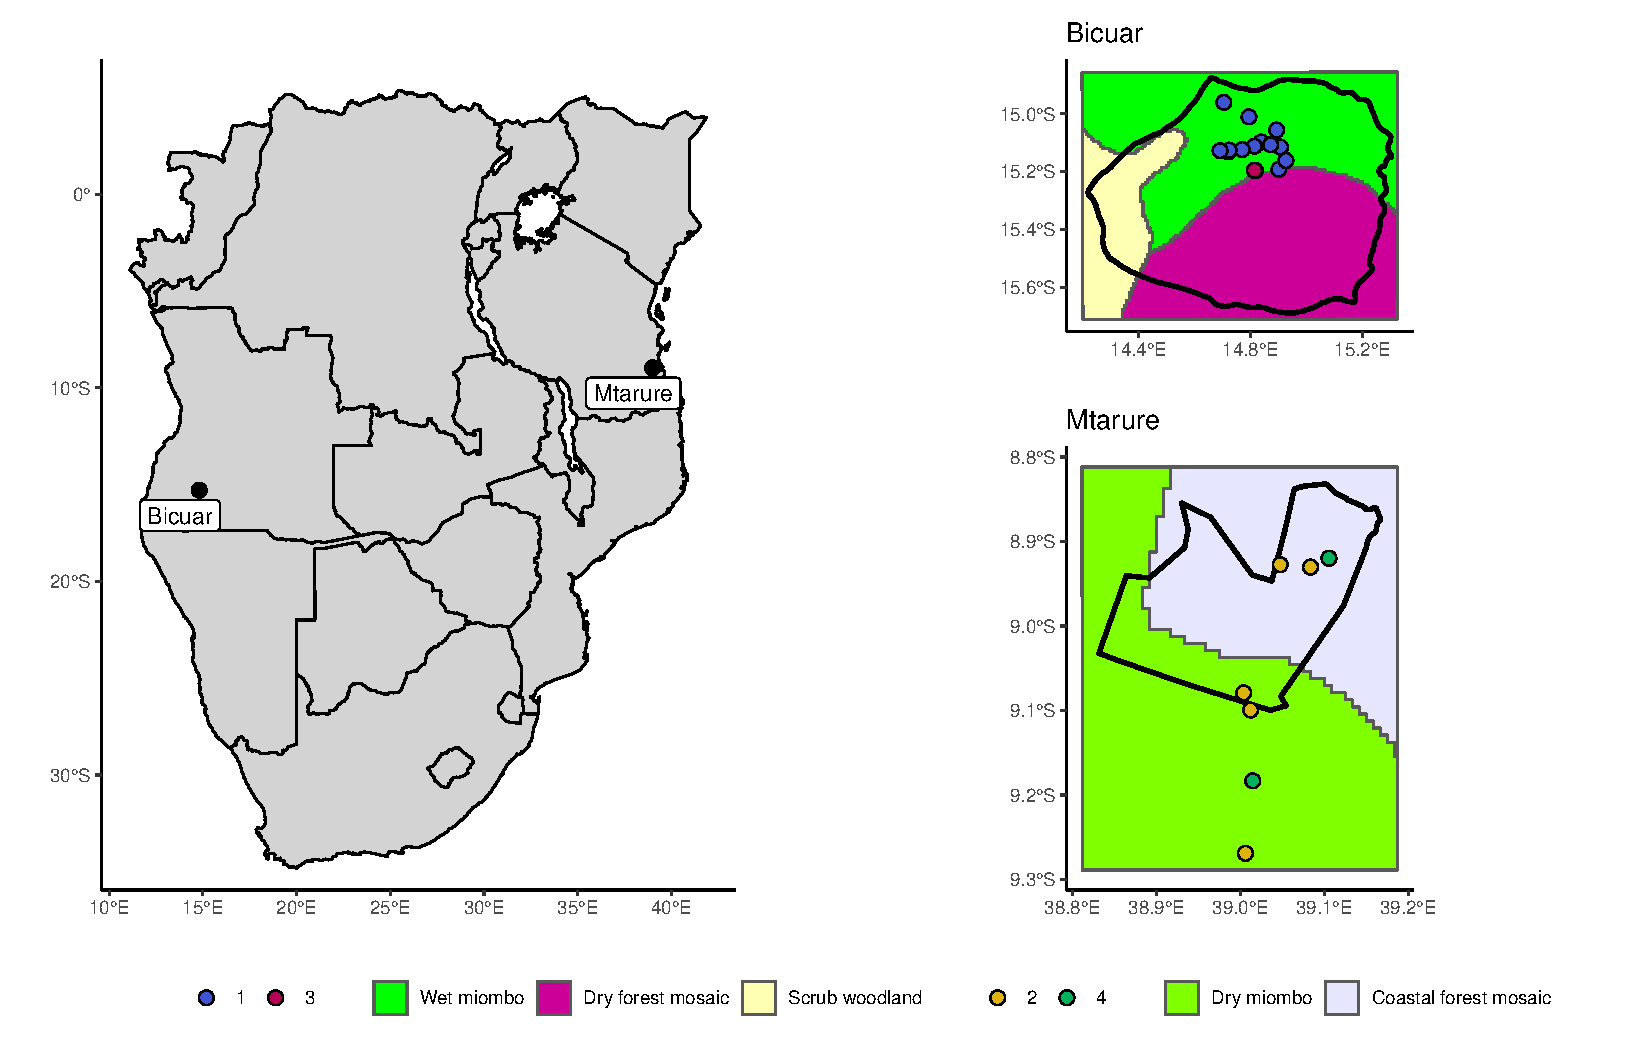
\includegraphics[width=\linewidth]{img/map}
	\caption[Maps of study sites and plots]{Location of study sites within southern Africa (left), and of 1 ha plots within each site (right). The black outlines in each site map denote the boundaries of protected areas which encompass the majority of study sites, Bicuar National Park in Angola (top), and Mtarure Forest Reserve in Tanzania (bottom). The background of each site map is a re-classified version of White's vegetation map \citep{White1983}. Points in site maps are shaded according to vegetation type identified by hierarchical clustering of tree genera abundances. Note that all maps are on different scales.}
	\label{tls:map}
\end{figure}

\subsection{Field measurements}
\label{tls:ssec:field}

Within each 1 ha plot, each woody stem $\geq$5 cm stem diameter was identified to species, the stem Diameter at Breast Height (DBH) was measured at 1.3 m above the ground, and the stem location within the plot was recorded using tape measures. Each 1 ha plot was sampled by nine 10 m diameter circular subplots arranged in a regular grid, with a 15 m buffer from the plot edge and 35 m between subplots. For each subplot, the distance and direction from the subplot centre of each stem >5 cm diameter with canopy material inside the subplot was recorded. Within each subplot, a variable number of scans were recorded using a Leica HDS6100 phase-shift Terrestrial Laser Scanner (TLS). The number and position of scans within a subplot was determined by the arrangement of canopy material in the subplot, to minimise shadows within the canopy of the subplot, and to maximise canopy penetration \citep{Beland2021b}. The number of scans per subplot ranged between one and five across both sites. Extended field methods and data analysis methods are described in \autoref{ch:workflow}.

\subsection{Data analysis}
\label{tls:ssec:analysis}

\subsubsection{TLS processing}
\label{tls:sssec:tls_process}

Point clouds from scans in each subplot were registered and unified using Leica Cyclone (version 9.1), with five reflective cross targets visible to all scans used as anchor points. Point clouds were voxelised to cubic voxels of different sizes depending on the application of the data. Subplot height profiles and canopy closure estimates  were calculated using 5 cm\textsuperscript{3} voxels, while whole plot canopy rugosity and canopy surface roughness were calculated using 50 cm\textsuperscript{3} voxels. Voxels were classified as `filled' if they intersected one or more points. Variation in voxel size reflects the spatial scale of each analysis, and is bounded by the beam divergence of the scanner over longer distances \citep{Cifuentes2014}. Choosing voxels that are too small can result in pock-marked representations of surfaces that are especially problematic when calculating larger scale canopy complexity metrics such as canopy top roughness, while voxels that are too large can result in an over-estimation of plant volume when estimating canopy foliage density at the subplot scale \citep{Seidel2012, Cifuentes2014}. 

The noise reduction algorithm from \citet{Rusu2008} was used to discard points based on mean nearest neighbour distances, with a number of neighbours of eight, and a standard deviation threshold of 1.96. This effectively removed `ghost points' produced by partial beam interceptions and also removed many erroneous returns caused by airborne dust particles, which was common at these study sites. Raw points clouds for each subplot had a mean of \textasciitilde{}\rawpt{} points, \textasciitilde{}\voxelpt{} points after voxelisation to 5 cm\textsuperscript{3}, and \textasciitilde{}\subpt{} points after noise reduction. 

Ground points were classified using the Progressive Morphological Filter (PMF) from \citet{Zhang2003}. Point cloud height was reclassified based on this revised ground layer by measuring the vertical distance between the nearest ground point and each point. Points below 1.3 m height above ground were discarded for calculations of foliage density, canopy cover, and canopy complexity, as points below this threshold were often occupied by long grass.

\subsubsection{Canopy complexity metrics}
\label{tls:sssec:canopy_metrics}

Ray-tracing was used to estimate canopy closure in each subplot, i.e. the proportion of the sky hemisphere occluded by plant material at the subplot centre from multiple TLS scans. Hemispherical images were created using the POV-Ray ray-tracing software \citep{Povray2004}. Filled voxels were represented as black cubes filling the voxel volume, with a white sky box and no light source. A `camera' with a 180\textdegree{} fisheye lens was placed at the subplot centre within POV-Ray, at a height of 1.3 m pointing directly upwards. The images produced by POV-Ray were analysed using Hemiphot to estimate canopy closure \citep{HemiPhot}. Canopy closure estimates from the TLS were validated with hemispherical photographs taken at the same location and processed using the same method in Hemiphot, and compared using Pearson's correlation (\hemiCor{}). A plot level estimate of canopy closure was calculated as the mean of subplot canopy closure measurements. See \autoref{ch:workflow} for expanded methods and explanation of the behaviour of the different canopy complexity metrics.

Effective Number of Layers (ENL) was calculated according to \citet{Ehbrecht2016} to measure vertical variation in subplot foliage density. ENL is calculated as the exponential Shannon index (i.e. the Hill number of order $q=1$) of foliage density among 50 cm vertical layers within each subplot:

\begin{equation}
	\text{ENL} = \exp\Big(-\sum_{i=1}^{N} p_{i} \times \ln p_{i} \Big)
\end{equation}

Where $p_{i}$ is the proportion of filled voxels in the 50 cm layer $i$, and $N$ is the total number of layers. ENL increases with canopy height and thus with number of layers, and also with variation in foliage density among those layers, but not with increased total foliage density.

Total foliage density was calculated within each subplot as the area under the curve of the foliage height profile. Total foliage density was also calculated at the plot level as the sum of filled 50 cm\textsuperscript{3} voxels across the plot. Vertical variation in subplot foliage density was calculated by fitting a linear model to the cumulative foliage density profile, then calculating the sum of squared residuals of that model. If foliage was distributed evenly throughout the vertical canopy profile, the residuals from the linear model would be zero, while clumping of foliage would cause departures from a linear cumulative foliage density profile.

Plot level canopy surface models were extracted using the 99th percentile of canopy height in 10 cm\textsuperscript{2} columns. A pit-filling algorithm provided by \citet{Khosravipour2014} was applied at 50 cm\textsuperscript{2} resolution to reduce the effects of incomplete canopy penetration in dense canopies. Whole plot canopy complexity was measured by three metrics. Canopy top roughness was measured as the coefficient of variation (CV) of canopy surface height across the plot. Canopy rugosity was measured according to \citet{Hardiman2011}, as the CV of vertical and horizontal foliage density within 50 cm\textsuperscript{3} cubic bins. Finally, canopy height was calculated as the mean of the canopy surface model across the plot.

\subsubsection{Stand structure and diversity}
\label{tls:sssec:structure_metrics}

An adapted version of the iterative Hegyi index was used to estimate crowding at the subplot scale. The iterative Hegyi index was used as an alternative to stem density, which does not adequately capture crowding at small spatial scales when only a small number of trees are included in the sample \citep{Hegyi1974}. The CV of stem basal area was calculated as a measure of the heterogeneity of tree size in the subplot neighbourhood. The iterative Hegyi index positively scales with stem diameter, number of stems, and the proximity of stems to the sample point (\autoref{ch:workflow}).

At the plot level, the regularity of species spatial distribution was estimated using the spatial mingling index \citep{Gadow2002}, which scores each tree based on whether it shares species identity with its nearest neighbours. The spatial regularity of tree location was estimated using the uniform angle index (winkelmass) \citep{Gadow2002}, which scores each tree based on the angles between nearest neighbours. Additionally, the degree of spatial clustering of trees was measured using Voronoi tessellation of tree locations, as the CV of Voronoi cell areas \citep{Ong2012}. Voronoi cell area CV increases as the spatial clustering of trees increases (\autoref{ch:workflow}). Finally, plot level tree density was calculated to estimate crowding at the plot scale. See \autoref{ch:workflow} for more information on the behaviour of the spatial mingling index, uniform angle index, and Voronoi cell area CV.

Species diversity at both the subplot and plot level was measured using the exponential Shannon index (i.e. the Hill number of order $q=1$), calculated using tree species abundances \citep{Hill1973, Jost2006}. At the subplot level trees were included if they had canopy material inside the 10 m diameter subplot, while at the plot level trees were included if the base of the largest stem was inside the plot boundaries.

\subsubsection{Statistical analysis}
\label{tls:sssec:stats}

Non-metric Multi-dimensional Scaling (NMDS) was used to describe variation in species composition among plots, using genus-level basal area weighted abundance in each plot. Trees that could not be identified to genus were excluded from this analysis, which accounted for \perIndet{}\% of the total basal area recorded. Four distinct vegetation types, two from each site (\autoref{tls:clust_summ}), were identified using hierarchical clustering of the four dominant NMDS ordination axes using Ward's algorithm. Clusters were further described using Dufr\^{e}ne-Legendre indicator species analysis and by ranking tree species according to abundance across all plots within each cluster. 

Linear mixed effects models tested the effects of tree species diversity and stand structural diversity on subplot canopy complexity metrics. Mixed models used a nested random intercept structure to account for the sampling design of subplots within plots and plots within vegetation types. Separate models were fitted for each canopy complexity metric, resulting in four models at the subplot level. Effect sizes among fixed effects in maximal models were compared for each canopy complexity metric, using the 95\% confidence interval of the effect size to ascertain the significance of fixed effects by whether the confidence interval overlapped zero \citep{Nakagawa2007}. AIC values and Akaike weights of models with different combinations of fixed effects were compared to determine which combination of diversity and structural metrics best explained variation in each canopy complexity metric. 

Statistical analysis of the determinants of plot level canopy complexity metrics were conducted using linear models. The ex-Acacia vegetation type was represented by only two plots and could not be included in this model due to lack of replication. As with the subplot linear mixed models, predictor variable effect sizes were used to assess predictor variable significance, and comparison of candidate models using AIC, Akaike weights, and model R\textsuperscript{2} values was used to determine which combination of predictors best explained each canopy complexity metric.

Path analysis was used to test whether tree species diversity influences canopy complexity indirectly through its effect on stand structure, using the \texttt{piecewiseSEM} R package \citep{piecewiseSEM}. Two path analyses were conducted, one at the plot level and one at the subplot level. Subplot path analysis investigated the direct effect of species diversity on canopy closure, as well as the indirect effect of diversity on canopy closure via the CV of basal area, with random intercept terms for each vegetation type. Again, these models excluded the ex-Acacia vegetation type due to lack of replication. Plot level path analysis investigated the direct effects of species diversity and spatial mingling of species on mean canopy height, as well as the indirect effects of these metrics on canopy height via tree density and basal area CV. Again, ex-Acacia plots were excluded from this path analysis.


% latex table generated in R 4.1.0 by xtable 1.8-4 package
% Fri Aug 27 10:03:30 2021
\begin{table}[]
\centering
\caption[Vegetation type descriptions]{Description of the vegetation type clusters, identified using Ward's algorithm based on basal area weighted genus abundance. AGB = Above-Ground woody Biomass. Species richness, stem density and AGB are reported as the median among plots, with the interquartile range in parentheses.} 
\label{tls:clust_summ}
\begin{tabular}{lcS[table-format=2.0]rrr}
  \toprule
{Site} & {Cluster} & {N sites} & {Richness} & \thead{Stem density\\(stems ha\textsuperscript{-1})} & \thead{AGB\\(t ha\textsuperscript{-1})} \\ 
  \midrule
Bicuar & 1 & 12 & 17(2) & 642(194) & 41( 8.4) \\ 
  Mtarure & 2 & 5 & 23(4) & 411(137) & 72(11.9) \\ 
  Bicuar & 3 & 3 &  6(1) & 196( 55) & 77( 7.3) \\ 
  Mtarure & 4 & 2 & 12(2) & 288( 73) &  9( 0.2) \\ 
   \bottomrule
\end{tabular}
\end{table}



\begin{landscape}
% latex table generated in R 4.1.0 by xtable 1.8-4 package
% Fri Aug 27 10:03:31 2021
\begin{table}
\centering
\caption[Floristic description of vegetation types]{Floristic description of the vegetation type clusters. Dominant species are the most abundant individuals across all plots within each cluster. Indicator species are the three species with the highest indicator values, from Dufr\^{e}ne-Legendre indicator species analysis.} 
\label{tls:indval}
\begin{tabular}{crrS[table-format=1.2]}
  \toprule
{Cluster} & {Dominant species} & {Indicator species} & {\thead{Indicator\\value}} \\ 
  \midrule
{\multirow{3}{*}{1}} & Julbernardia paniculata & Strychnos spinosa & 0.83 \\ 
   & Burkea africana & Combretum collinum & 0.74 \\ 
   & Combretum collinum & Julbernardia paniculata & 0.70 \\ 
   \midrule
{\multirow{3}{*}{2}} & Diplorhynchus condylocarpon & Pteleopsis myrtifolia & 1.00 \\ 
   & Pseudolachnostylis maprouneifolia & Diplorhynchus condylocarpon & 0.89 \\ 
   & Gymnosporia senegalensis & Pseudolachnostylis maprouneifolia & 0.81 \\ 
   \midrule
{\multirow{3}{*}{3}} & Baikiaea plurijuga & Baikiaea plurijuga & 0.94 \\ 
   & Baphia massaiensis & Baphia massaiensis & 0.83 \\ 
   & Philenoptera nelsii & Philenoptera nelsii & 0.45 \\ 
   \midrule
{\multirow{3}{*}{4}} & Combretum apiculatum & Vachellia nilotica & 0.99 \\ 
   & Burkea africana & Combretum apiculatum & 0.70 \\ 
   & Bauhinia petersiana & Senegalia polyacantha & 0.62 \\ 
   \bottomrule
\end{tabular}
\end{table}


\end{landscape}

\section{Results}
\label{tls:sec:results}

\subsection{Description of vegetation types}
\label{tls:ssec:veg_types}

Indicator species analysis shows that the four vegetation types identified by hierarchical clustering constitute common southern African savanna floristic archetypes (\autoref{tls:indval}). Cluster 1, found in Bicuar National Park contains typical miombo species from the Detarioideae subfamily, such as \textit{Julbernardia paniculata}. Cluster 1 is the most frequent vegetation type in this study, with 12 plots. Cluster 1 has the highest stem density, but lower Above-Ground woody Biomass (AGB) than Clusters 2 or 3, which contain larger individuals with disproportionately higher biomass. Cluster 2, found in Mtarure Forest Reserve, is dominated by \textit{Pteleopsis myrtifolia}, a common miombo species from the Combretaceae family. Indeed, Cluster 2 also contained other common miombo species shared with plots in Cluster 1, such as \textit{Julbernardia globiflora} and \textit{Pseudolachnostylis maprouneifolia}, but these clusters remain distinct due to biogeographic variation in endemic genera at the longitudinal extremes of the miombo ecoregion represented by the two sites in this study. Cluster 3 represents \textit{Baikiaea} woodland, found on Kalahari sands in southern Angola. It is species poor and dominated by \textit{Baikiaea plurijuga} which forms large spreading canopy trees with high AGB. Other shrubby species that coppice readily in response to disturbance by fire such as \textit{Baphia massaiensis} are also common. Cluster 4, found in Mtarure is a type of ex-Acacia woodland, dominated by \textit{Vachellia} and \textit{Senegalia} spp. This vegetation type was not well represented in the study, with only two plots, precluding its use in some multi-level statistical analyses at the plot level due to lack of replication. Cluster 4 had far lower AGB than the other clusters (\autoref{tls:clust_summ}). 

Differences in canopy structure among the four vegetation types are evident through observation of canopy surface models for typical plots within each vegetation type (\autoref{tls:veg_type_tile}), and by comparing canopy complexity metrics (\autoref{tls:canopy_metric_box}). Cluster 1 shows many overlapping crowns forming a nearly contiguous canopy surface, and the highest plot foliage density of all clusters. Though the tallest trees in Cluster 1 have smaller crowns than those in Cluster 2, which also forms a nearly contiguous canopy. The largest trees in Cluster 2 grow taller and have a wider spreading canopy than those in other vegetation types. Cluster 3 shows two distinct size classes of tree, the large \textit{Baikiaea plurijuga} forming clear isolated canopies, and much smaller scattered shrubby individuals in the understorey. Cluster 4 shows many small shrubby individuals with irregular canopy shapes, but a greater total crown area coverage than Cluster 3. 

\begin{figure}
	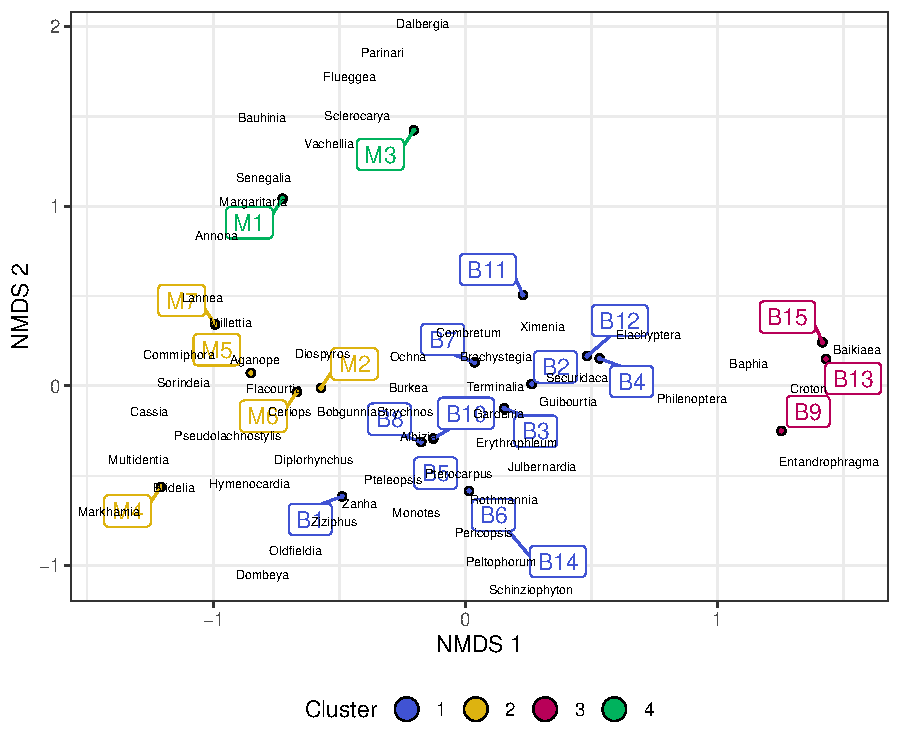
\includegraphics[width=\linewidth]{img/nmds}
	\caption[NMDS of plots based on genera basal area abundance]{The first two axes of a Non-metric Multi-Dimensional Scaling (NMDS) analysis of tree genus diversity in each plot. Genus scores are labelled as black text, while plot scores are labelled as coloured points. Plots are shaded by vegetation type, identified by hierarchical clustering: 1) B1-B8, B10-B12, B14, dominated by core miombo species such as \textit{Julbernardia} spp., \textit{Brachystegia} spp.; 2) M2, M5, M6, and M7, also dominated by core miombo genera with some genera not found in Bicuar National Park such as \textit{Commiphora} and \textit{Sorindeia}; 3) B9, B13 and B15, dominated by \textit{Baikiaea plurijuga}; and 4) M1, M3, and M4, dominated by \textit{Senegalia} spp., \textit{Vachellia} spp., and \textit{Combretum} spp.}
	\label{tls:nmds}
\end{figure}

\subsection{Bivariate relationships}
\label{tls:ssec:bivar}

Bivariate plots and linear models show that subplot species diversity, measured as the true-numbers equivalent of the Shannon diversity index of the tree neighbourhood around each 10 m diameter subplot, appears to have weak positive effects on subplot canopy layer diversity, canopy closure and foliage density (\autoref{tls:subplot_bivar}, \autoref{tls:bivar_lm_summ_all}). The Hegyi crowding index had strong positive effects on canopy closure and layer diversity, as expected. The effect of Hegyi crowding on subplot canopy complexity metrics was similar across all vegetation types (\autoref{tls:bivar_lm_summ_veg_type}). Structural diversity, measured as the CV of subplot stem basal area had significant weak positive effects on total canopy foliage, layer diversity, and canopy closure. 

At the plot level, effects of species diversity and stand structure on canopy complexity were similarly weak, but not strictly significant except for the effect on canopy height, which explained more variance in canopy height than tree density (\autoref{tls:bivar_lm_summ_all}, \autoref{tls:plot_bivar}). The effect of spatial regularity of trees on canopy closure, measured by uniform angle index, was clearly negative, while the effect of spatial clustering of stems, measured by Voronoi cell area CV, was negligible. Additionally, there was a non-significant negative effect of basal area CV on whole canopy rugosity. As expected, tree density had strong positive and significant effects on foliage density and canopy closure, but negative effects on canopy roughness and canopy rugosity. Cluster 4 represented an outlier in plot level bivariate relationships, with low canopy closure, low canopy height, low species diversity, and low variation in stem size.

% latex table generated in R 4.1.0 by xtable 1.8-4 package
% Fri Aug 27 10:40:49 2021
\begin{longtable}{llcccS[table-format=-2.2, table-space-text-post = {***}]}
\caption[Bivariate linear model summary]{Summary statistics of bivariate linear models comparing canopy complexity metrics with diversity and stand structural metrics across all vegetation types. Slope refers to the slope of the predictor term in the model, $\pm$1 standard error. T is the t-value of the slope of the predictor term in the model, Asterisks indicate the p-value of these terms (***<0.001, **<0.01, *<0.05).} 
\label{tls:bivar_lm_summ_all} \\
\toprule
{Response} & {Predictor} & {Slope} & {F} & {R\textsuperscript{2}} & {T} \\ 
\midrule
\endfirsthead
\toprule
{Response} & {Predictor} & {Slope} & {F} & {R\textsuperscript{2}} & {T} \\ 
\midrule
\endhead
{\multirow{3}{*}{Foliage density}} & Basal area CV &  8.7e+01$\pm$3.0e+01 & 8.6(2,167) & 0.05 & 2.93** \\* 
   & Hegyi &  7.8e+03$\pm$1.6e+03 & 25.5(2,184) & 0.12 & 5.05*** \\* 
   & Shannon &  3.2e+03$\pm$1.1e+03 & 8.9(2,180) & 0.05 & 2.98** \\ 
   \midrule
{\multirow{3}{*}{Canopy closure}} & Basal area CV &  1.2e-03$\pm$4.8e-04 & 6.3(2,168) & 0.04 & 2.52* \\* 
   & Hegyi &  2.4e-01$\pm$2.1e-02 & 132.8(2,185) & 0.42 & 11.52*** \\* 
   & Shannon &  4.7e-02$\pm$1.7e-02 & 7.3(2,181) & 0.04 & 2.70** \\ 
   \midrule
{\multirow{3}{*}{Foliage uniformity}} & Basal area CV &  4.1e+00$\pm$3.0e+00 & 1.9(2,167) & 0.01 & 1.37 \\* 
   & Hegyi &  4.0e+02$\pm$1.6e+02 & 6.2(2,184) & 0.03 & 2.49* \\* 
   & Shannon &  2.2e+02$\pm$1.1e+02 & 4.1(2,180) & 0.02 & 2.04* \\ 
   \midrule
{\multirow{3}{*}{Layer diversity}} & Basal area CV &  3.2e-02$\pm$7.6e-03 & 17.6(2,167) & 0.10 & 4.20*** \\* 
   & Hegyi &  2.7e+00$\pm$3.9e-01 & 46.8(2,184) & 0.20 & 6.84*** \\* 
   & Shannon &  1.1e+00$\pm$2.7e-01 & 16.8(2,180) & 0.09 & 4.10*** \\ 
   \midrule
{\multirow{6}{*}{Canopy roughness}} & Basal area CV &  3.0e-02$\pm$5.0e-02 & 0.4(2,16) & 0.02 & 0.60 \\* 
   & Voronoi CV &  7.5e-01$\pm$5.9e-01 & 1.6(2,16) & 0.09 & 1.26 \\* 
   & Mingling & -2.8e+01$\pm$3.3e+01 & 0.7(2,16) & 0.04 & -0.86 \\* 
   & Tree density & -2.6e-02$\pm$1.7e-02 & 2.3(2,16) & 0.12 & -1.51 \\* 
   & Shannon & -1.9e+00$\pm$9.5e-01 & 4.0(2,16) & 0.20 & -2.01 \\* 
   & Uniform angle index &  1.6e+02$\pm$1.6e+02 & 1.0(2,16) & 0.06 & 0.98 \\ 
   \midrule
{\multirow{6}{*}{Canopy height}} & Basal area CV &  7.1e-03$\pm$7.3e-03 & 0.9(2,16) & 0.06 & 0.97 \\* 
   & Voronoi CV & -4.7e-02$\pm$9.1e-02 & 0.3(2,16) & 0.02 & -0.52 \\* 
   & Mingling &  3.8e+00$\pm$4.8e+00 & 0.6(2,16) & 0.04 & 0.79 \\* 
   & Tree density &  4.3e-03$\pm$2.5e-03 & 3.1(2,16) & 0.16 & 1.76 \\* 
   & Shannon &  3.3e-01$\pm$1.3e-01 & 6.0(2,16) & 0.27 & 2.45* \\* 
   & Uniform angle index & -2.2e+01$\pm$2.4e+01 & 0.8(2,16) & 0.05 & -0.90 \\ 
   \midrule
{\multirow{6}{*}{Canopy closure}} & Basal area CV &  8.5e-04$\pm$5.7e-04 & 2.2(2,20) & 0.10 & 1.50 \\* 
   & Voronoi CV &  2.4e-03$\pm$5.8e-03 & 0.2(2,20) & 0.01 & 0.41 \\* 
   & Mingling &  7.2e-03$\pm$3.7e-01 & 0.0(2,20) & 0.00 & 0.02 \\* 
   & Tree density &  4.7e-04$\pm$1.9e-04 & 6.3(2,20) & 0.24 & 2.50* \\* 
   & Shannon &  1.0e-02$\pm$1.2e-02 & 0.7(2,20) & 0.04 & 0.86 \\* 
   & Uniform angle index & -3.4e+00$\pm$1.7e+00 & 3.9(2,20) & 0.16 & -1.98 \\ 
   \midrule
{\multirow{6}{*}{Foliage density}} & Basal area CV &  5.8e+01$\pm$3.2e+01 & 3.3(2,16) & 0.17 & 1.80 \\* 
   & Voronoi CV &  5.8e+02$\pm$4.1e+02 & 2.1(2,16) & 0.11 & 1.43 \\* 
   & Mingling &  6.6e+03$\pm$2.3e+04 & 0.1(2,16) & 0.01 & 0.29 \\* 
   & Tree density &  3.0e+01$\pm$1.0e+01 & 8.6(2,16) & 0.35 & 2.93** \\* 
   & Shannon &  1.1e+03$\pm$6.9e+02 & 2.5(2,16) & 0.13 & 1.57 \\* 
   & Uniform angle index & -2.1e+04$\pm$1.1e+05 & 0.0(2,16) & 0.00 & -0.18 \\ 
   \midrule
{\multirow{6}{*}{Canopy rugosity}} & Basal area CV & -1.0e+00$\pm$5.3e-01 & 3.7(2,16) & 0.19 & -1.92 \\* 
   & Voronoi CV & -6.0e+00$\pm$7.0e+00 & 0.7(2,16) & 0.04 & -0.86 \\* 
   & Mingling &  1.3e+02$\pm$3.8e+02 & 0.1(2,16) & 0.01 & 0.33 \\* 
   & Tree density & -5.2e-01$\pm$1.7e-01 & 10.0(2,16) & 0.38 & -3.16** \\* 
   & Shannon & -1.3e+01$\pm$1.2e+01 & 1.2(2,16) & 0.07 & -1.11 \\* 
   & Uniform angle index & -1.8e+03$\pm$1.9e+03 & 0.9(2,16) & 0.06 & -0.97 \\ 
   \bottomrule
\end{longtable}



\begin{figure}
	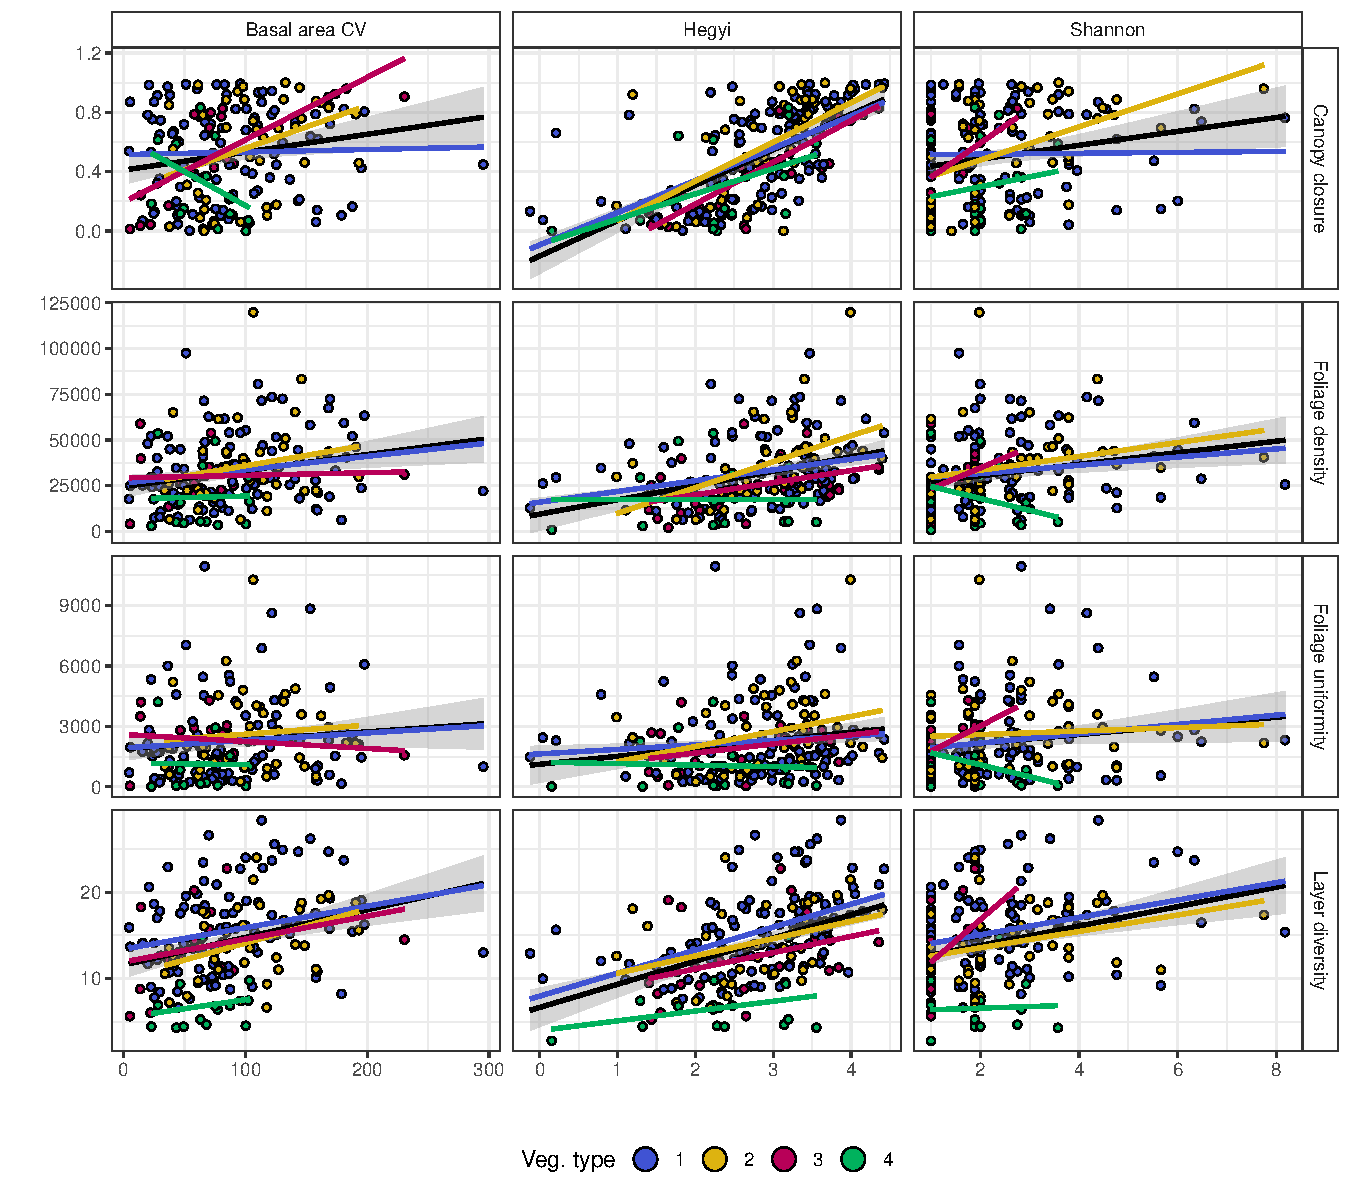
\includegraphics[width=\linewidth]{img/bivar_subplot}
	\caption[Bivariate plots comparing diversity, stand structure and canopy complexity]{Subplot level bivariate relationships between diversity/stand structure metrics (x axis) and canopy complexity metrics (y axis). Points and linear model lines of best fit are coloured by vegetation type. Black lines of best fit are linear models including all plots, with a 95\% confidence interval. See \autoref{tls:bivar_lm_summ_veg_type} for a comparison of linear model fits by vegetation type.}
	\label{tls:subplot_bivar}
\end{figure}

\begin{landscape}
\begin{figure}
	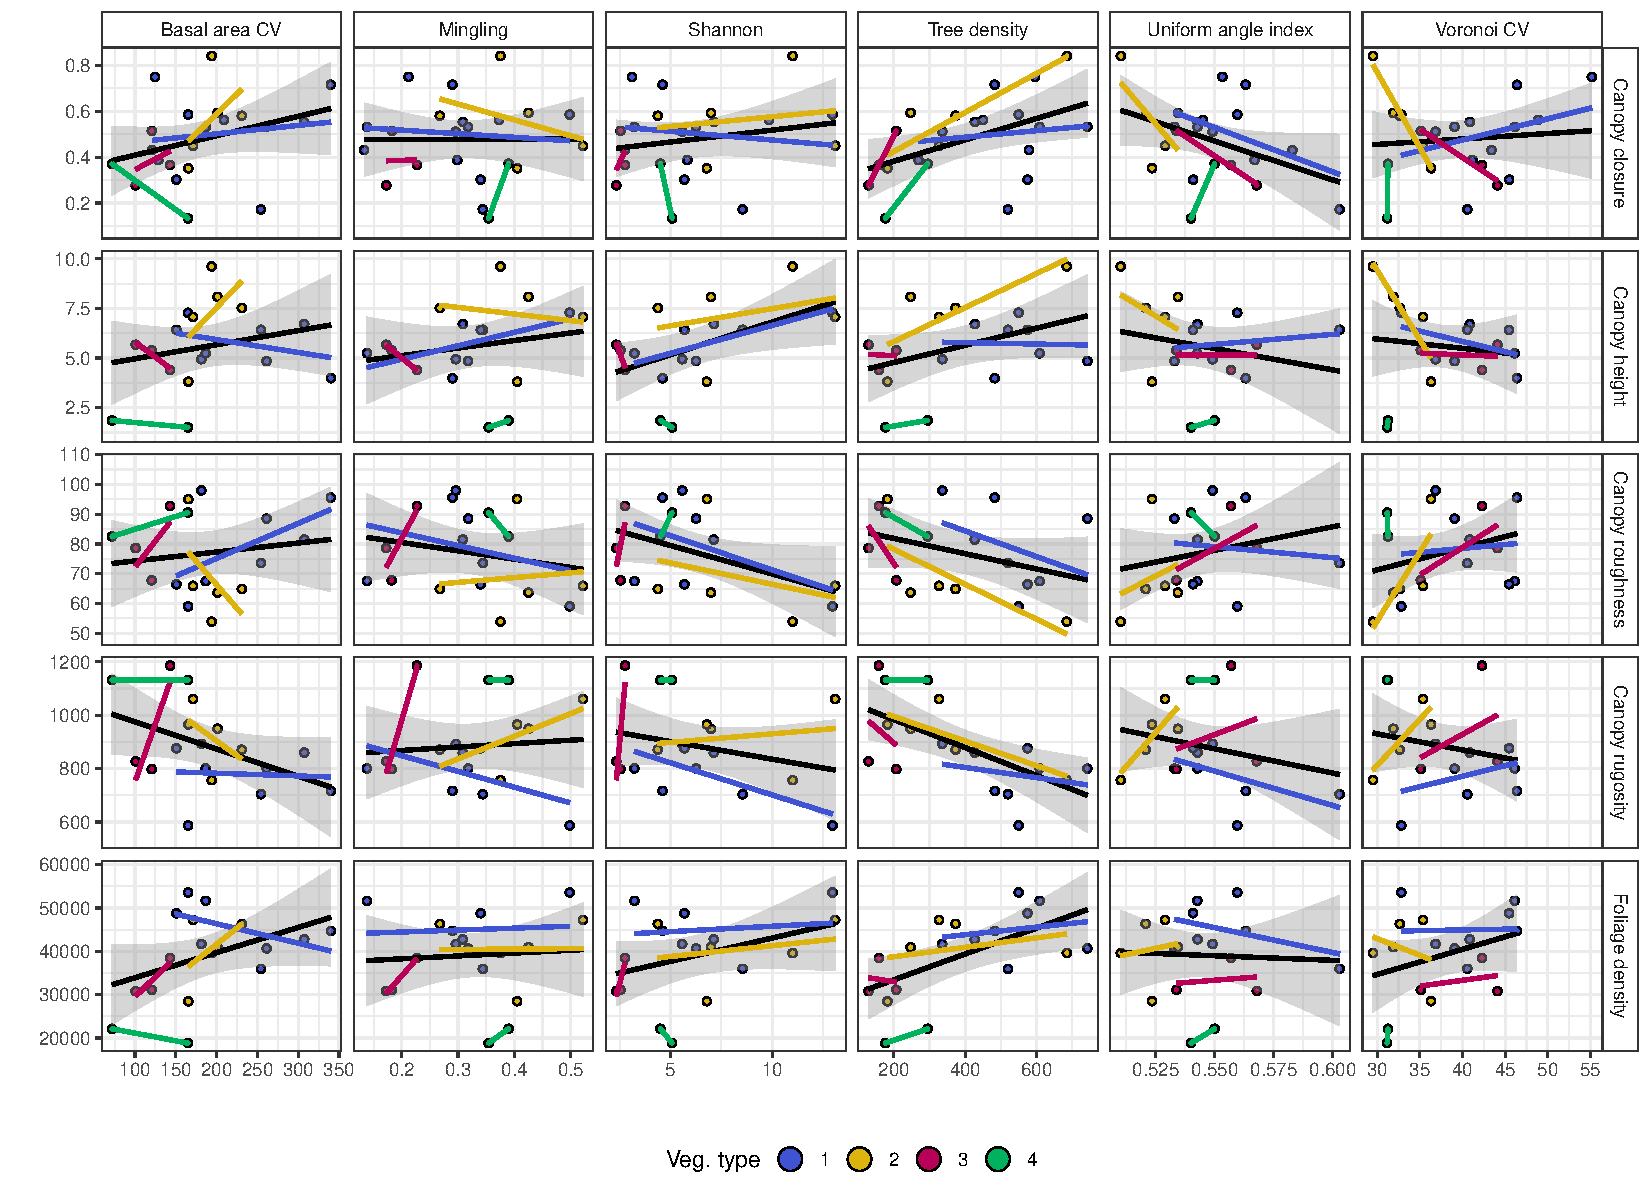
\includegraphics[width=0.8\linewidth]{img/bivar_plot}
	\caption[Bivariate plots comparing diversity, stand structure and canopy complexity]{Plot level bivariate relationships between diversity/stand structure metrics (x axis) and canopy complexity metrics (y axis). Points and linear model lines of best fit are coloured by vegetation type. Black lines of best fit are linear models including all plots, with a 95\% confidence interval. See \autoref{tls:bivar_lm_summ_veg_type} for a comparison of linear model fits by vegetation type.}
	\label{tls:plot_bivar}
\end{figure}
\end{landscape}


\begin{figure}
	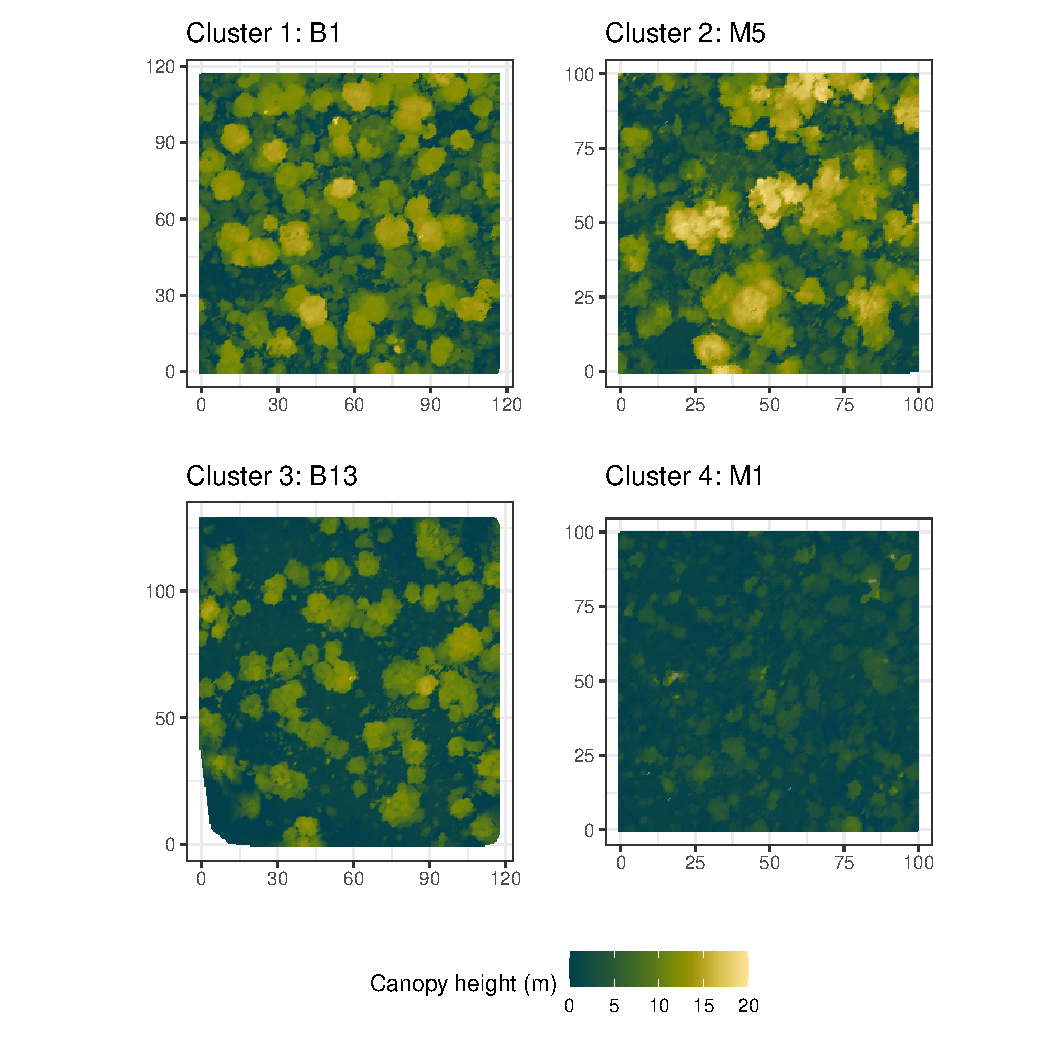
\includegraphics[width=\linewidth]{img/veg_type_tile}
	\caption[Canopy surface models]{Representative canopy surface models for each vegetation type identified in the hierarchical clustering analysis. Panel titles show the plot name and the vegetation type cluster.}
	\label{tls:veg_type_tile}
\end{figure}

\begin{figure}
	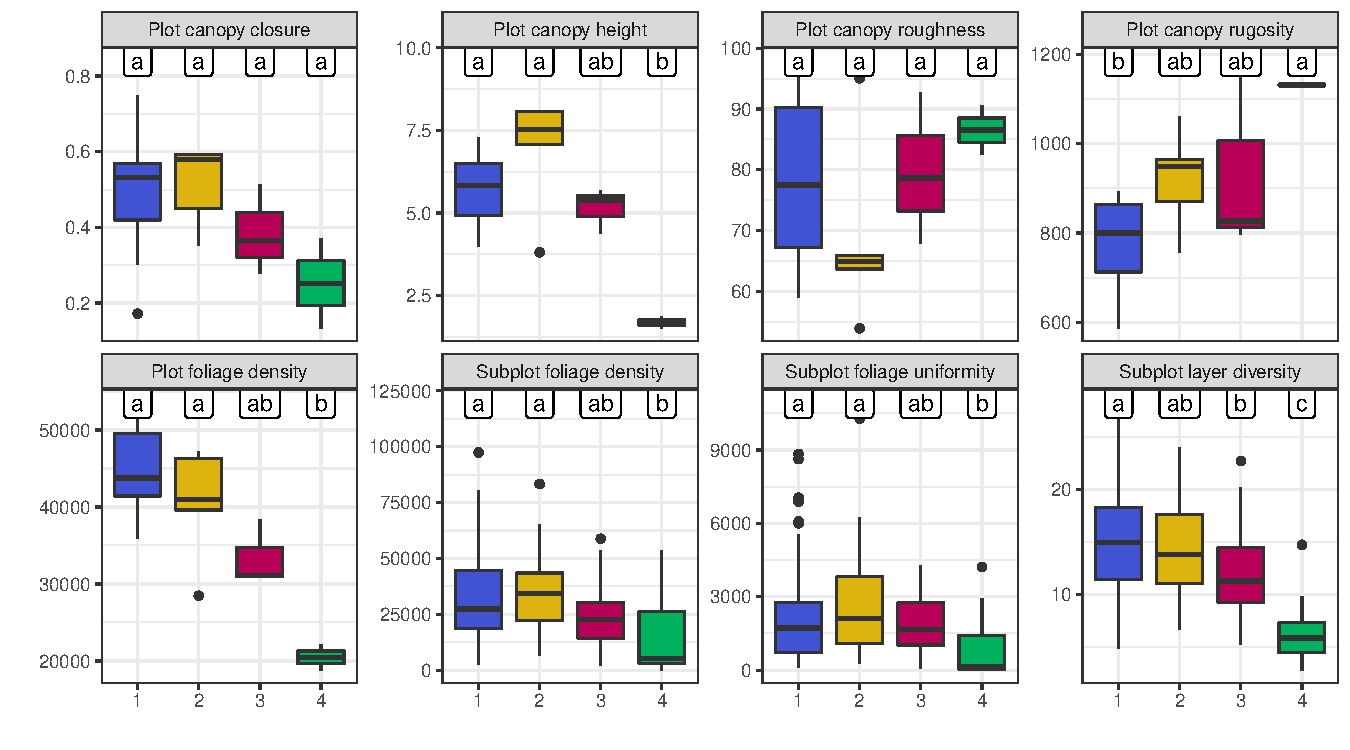
\includegraphics[width=\linewidth]{img/canopy_metric_box}
	\caption[Boxplots of canopy complexity metrics]{Box plots showing variation in canopy complexity metrics among the four vegetation types identified in the hierarchical clustering analysis. Thick lines show the median, boxes show the interquartile range (IQR), whiskers show 1.5$\times$IQR, and points show outliers beyond these limits. Labels above each box plot group vegetation types according to significant differences in pairwise Tukey's tests; vegetation types sharing a letter are not significantly different.}
	\label{tls:canopy_metric_box}
\end{figure}

\subsection{Subplot mixed models}
\label{tls:ssec:subplot_models}

Linear mixed effects models showed that species diversity of the subplot neighbourhood contributed to both layer diversity and canopy closure (\autoref{tls:height_profile_sig_vars_dredge}), despite their low R\textsuperscript{2} in bivariate linear models (\autoref{tls:bivar_lm_summ_all}), and low effect sizes in maximal linear mixed models (\autoref{tls:height_profile_mod_rich_slopes_sites}). As also seen in the subplot bivariate relationships (\autoref{tls:subplot_bivar}), the Hegyi crowding index had strong positive effects on canopy closure and layer diversity, though these effects were non-significant for vegetation Clusters 3 and 4. Stem basal area CV had a significant positive effect on layer diversity and foliage density, but there was wide variation in vegetation type marginal effects for Clusters 3 and 4, due to low levels of replication. Cluster 3 had strong positive effects of species diversity on foliage uniformity and layer diversity. The random effects of vegetation type and plot identity described most of the variation in layer diversity and foliage density. Foliage uniformity was poorly explained by all combinations of fixed effects, with the best model only explaining \bestUnifRsqS\%. All models were better than random effects only models according to AIC values (\autoref{tls:height_profile_sig_vars_dredge}).

\begin{figure}
	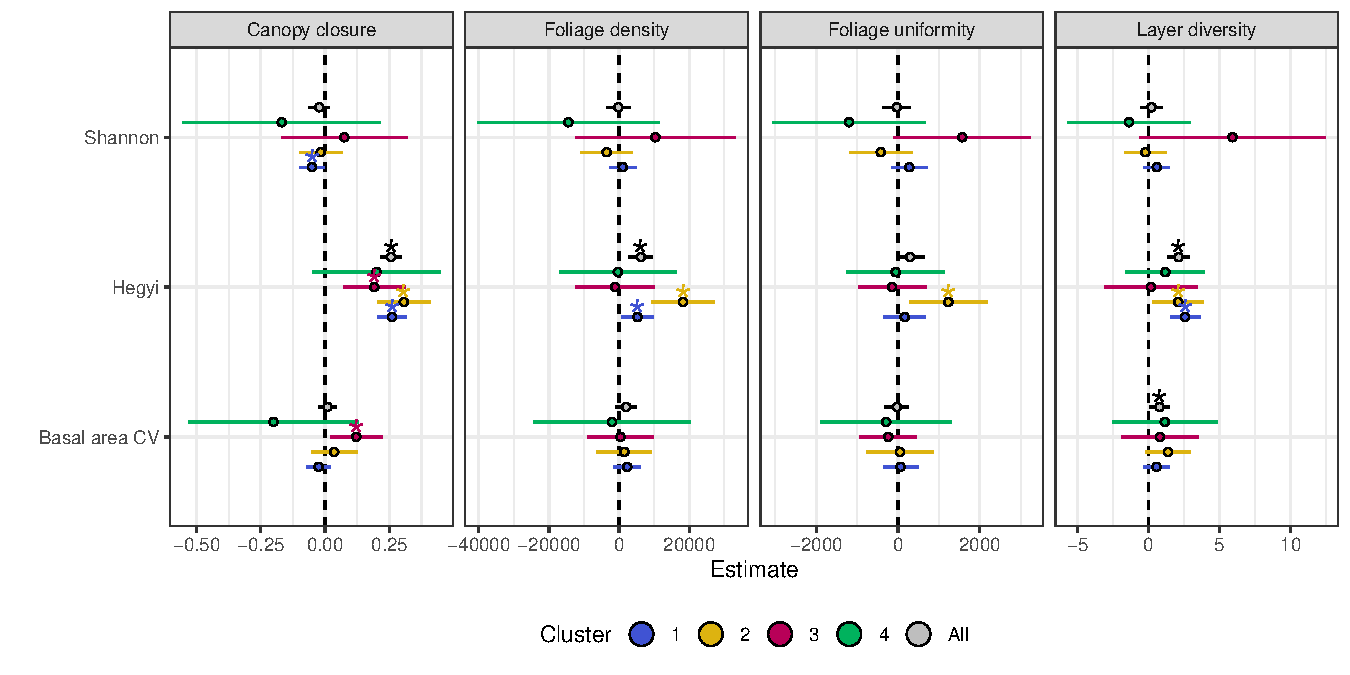
\includegraphics[width=\linewidth]{img/height_profile_mod_rich_slopes_sites}
	\caption[Subplot canopy complexity metric fixed effects]{Standardised fixed effect slopes for each subplot canopy complexity metric model metric. Slope estimates where the interval ($\pm$1 standard error) does not overlap zero are considered to be significant effects, marked with asterisks. Points are coloured according to vegetation type.}
	\label{tls:height_profile_mod_rich_slopes_sites}
\end{figure}

% latex table generated in R 4.1.0 by xtable 1.8-4 package
% Fri Aug 27 10:04:08 2021
\begin{table}[]
\centering
\caption[Model fit statistics for best subplot canopy complexity models]{Explanatory variables included in the best model for each subplot canopy complexity variable. $\Delta$AIC shows the difference in model AIC value compared to a null model which included only the random effects of vegetation type and plot. $\Delta$AIC values >2 indicate that the model is of better quality than the null model. R\textsuperscript{2}\textsubscript{c} is the R\textsuperscript{2} of the best model, while R\textsuperscript{2}\textsubscript{m} is the R\textsuperscript{2} of the model fixed effects only.} 
\label{tls:height_profile_sig_vars_dredge}
\begin{tabular}{lcccS[table-format=3.1]cc}
  \toprule
{Response} & {Hegyi} & {Shannon} & {\thead{Basal area\\CV}} & {$\Delta$AIC} & {R\textsuperscript{2}\textsubscript{c}} & {R\textsuperscript{2}\textsubscript{m}} \\ 
  \midrule
Layer diversity & \checkmark & \checkmark & \checkmark & 37.0 & 0.50 & 0.17 \\ 
  Foliage density & \checkmark &  & \checkmark & 47.6 & 0.27 & 0.09 \\ 
  Foliage uniformity & \checkmark &  &  & 13.1 & 0.28 & 0.02 \\ 
  Canopy closure & \checkmark & \checkmark &  & 101.9 & 0.60 & 0.46 \\ 
   \bottomrule
\end{tabular}
\end{table}



\subsection{Plot level linear models}
\label{tls:ssec:plot_models}

While species diversity had varying effects on different plot level canopy complexity metrics, the confidence intervals on these effect sizes were wide (\autoref{tls:canopy_rough_slopes}). Species diversity had a significant positive effect on canopy height (\shannonHeightP{}), a non-significant positive effect on canopy closure (\shannonCoverP{}), but a negative effect on canopy surface roughness (\shannonRoughP{}) and whole canopy rugosity (\shannonRugP{}). Spatial mingling of tree species had a positive effect on canopy surface roughness and canopy rugosity, but a negative effect on canopy height. Plot tree density had negligible effects on canopy complexity, except for canopy rugosity (\treeDensRugP{}), in contrast to the effect of Hegyi crowding on subplot canopy complexity. Measures of structural diversity, measured by the uniform angle index, Voronoi cell area CV, and basal area CV, had smaller effects on canopy complexity than species diversity, and were generally insignificant. One exception was the effect of uniform angle index, i.e. the spatial clustering of stems, on canopy closure, which was clearly negative, though still insignificant (\wiCoverP{}), the effect of Voronoi cell area CV on foliage density, which was positive (\voronoiDensP{}), and the effect of basal area CV on canopy closure, which was positive (\baCoverP{}). 

Despite the weak effect sizes of species diversity on canopy complexity at the plot level, model selection showed that foliage density, canopy height and canopy roughness were better explained by models which included species diversity (\autoref{tls:canopy_sig_vars_dredge}). Additionally, the best models for canopy height and canopy roughness also included spatial mingling of tree species. The model for canopy roughness was only marginally better than a null model and the model did not have a significant p-value.

\begin{figure}
	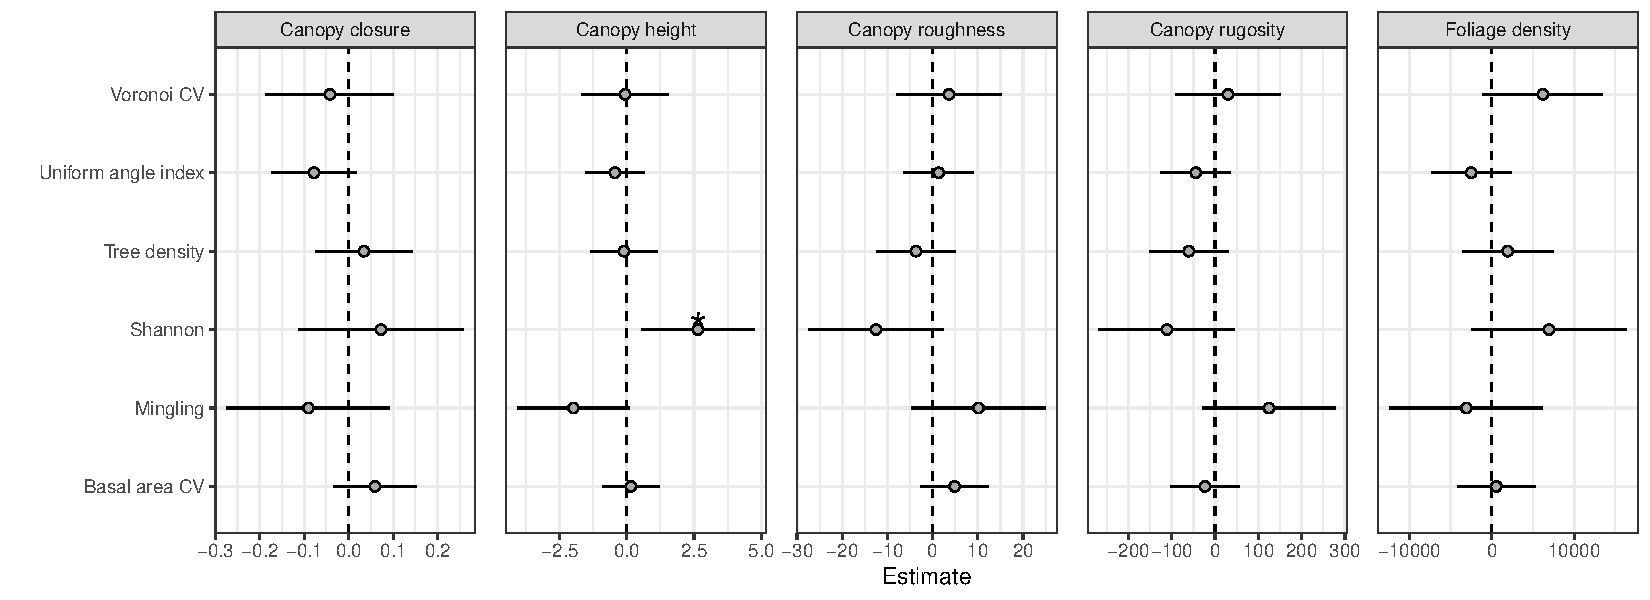
\includegraphics[width=\linewidth]{img/canopy_rough_slopes}
	\caption[Plot canopy complexity metric fixed effects]{Standardised effect sizes for whole-plot canopy rugosity. Slope estimates where the interval ($\pm$1 standard error) does not overlap zero are considered to be significant effects, marked with asterisks.}
	\label{tls:canopy_rough_slopes}
\end{figure}

\begin{landscape}
% latex table generated in R 4.1.0 by xtable 1.8-4 package
% Fri Aug 27 10:04:22 2021
\begin{table}[]
\centering
\caption[Model fit statistics for best plot canopy complexity models]{Explanatory variables included in the best linear model for each plot-level canopy complexity metric. $\Delta$AIC shows the difference in model AIC value compared to a null model. $\Delta$AIC values >2 indicate that the model is of better quality than the null model.} 
\label{tls:canopy_sig_vars_dredge}
\setlength{\tabcolsep}{3pt}
\begin{tabular}{lccccccccS[table-format=<1.2]}
  \toprule
{Response} & {Shannon} & {\thead{Tree\\density}} & {\thead{Basal area\\CV}} & {Mingling} & {\thead{Uniform\\angle index}} & {\thead{Voronoi\\CV}} & {$\Delta$AIC} & {R\textsuperscript{2}} & {Prob.} \\ 
  \midrule
Foliage density & \checkmark &  &  &  &  & \checkmark & 5.8 & 0.42 & <0.05 \\ 
  Canopy closure &  &  & \checkmark &  & \checkmark &  & 5.8 & 0.42 & <0.05 \\ 
  Canopy height & \checkmark &  &  & \checkmark &  &  & 8.2 & 0.49 & <0.01 \\ 
  Canopy roughness & \checkmark &  &  & \checkmark &  &  & 2.5 & 0.30 & 0.07 \\ 
  Canopy rugosity &  & \checkmark &  &  & \checkmark &  & 6.9 & 0.45 & <0.05 \\ 
   \bottomrule
\end{tabular}
\end{table}


\end{landscape}

\subsection{Path analysis}
\label{tls:ssec:path_analysis}

The subplot level path analysis investigating the indirect effect of subplot species diversity on canopy closure via the basal area CV showed that while species diversity had a strong positive significant effect on basal area variation, the effect of basal area variation on canopy closure remained negligible (\autoref{tls:path_diag_cover}). The indirect effect of species diversity on canopy closure via basal area CV was \shannonBaCoverPath{}, while the direct effect was \shannonCoverPath{}. The R\textsuperscript{2} of this model was \coverSemRm{}. As in the bivariate relationships and plot level linear models, species diversity had a weak positive significant effect on canopy closure, while the major driver of canopy closure was the Hegyi crowding index. 

The plot level path analysis, which tested the effects of species diversity and species mingling on canopy height, showed that the main effect of species diversity on canopy height was direct (\treeShannonHeightPath{}), while the indirect effects via basal area CV (\treeShannonBaHeightPath{}), and tree density (\treeShannonDensHeightPath{}), remained small and insignificant. Shannon diversity had a strong positive effect on tree density. Species mingling had a moderately strong negative but insignificant direct effect on canopy height, as in the linear mixed models and bivariate relationships.

\begin{figure}
	\begin{tikzpicture}[
	mybox/.style={
    	rectangle,
    	draw,
    	very thick,
    	inner sep=0pt,
    	minimum width=20mm,
    	minimum height=10mm,
    	text width=2cm,
		align=center
    },
    myarrow/.style={
    	thick,
    	-Stealth 
    },
    mypathnode/.style={
    	text width=1cm,
    	align=center,
    	fill=white
    }
]

\node [mybox] (A1) at (0,0) {Shannon};
\node [mybox] (B1) [above right=of A1] {Basal\\area CV};
\node [mybox] (C1) [below right=of B1] {Hegyi};
\node [mybox] (D1) [below right=of A1] {Canopy\\closure};

\path[myarrow] (A1.north) edge node[mypathnode] {\shannonBaPath} (B1.west); 
\path [myarrow] (C1.north) edge node[mypathnode] {\hegyiBaPath} (B1.east); 
\path [myarrow] (B1.south) edge node[mypathnode] {\baCoverPath} (D1.north); 
\path [myarrow] (A1.south) edge node[mypathnode] {\shannonCoverPath} (D1.west); 
\path [myarrow] (C1.south) edge node[mypathnode] {\hegyiCoverPath} (D1.east); 

\end{tikzpicture}


	\caption[Path coefficients for subplot canopy closure path analysis]{Directed Acyclic Graph showing standardised path coefficients of paths in the path analysis of the indirect effect of subplot species diversity (Shannon diversity index) on canopy closure via basal area CV. Asterisks define p-value thresholds: *<0.05, **<0.01, ***<0.001.}
	\label{tls:path_diag_cover}
\end{figure}

\begin{figure}
	\begin{tikzpicture}[
	mybox/.style={
    	rectangle,
    	draw,
    	very thick,
    	inner sep=2pt,
    	minimum width=2cm,
    	minimum height=1cm,
    	text width=2cm,
		align=center
    },
    myarrow/.style={
    	thick,
    	-Stealth 
    },
    mypathnode/.style={
    	text width=1.2cm,
    	align=center,
    	fill=white
    }
]

\node [mybox] (A1) at (0,0) {Canopy height};
\node [mybox] (B1) [above left=of A1] {Shannon};
\node [mybox] (C1) [above right=of A1] {Tree density};
\node [mybox] (D1) [below left=of A1] {Basal area CV};
\node [mybox] (E1) [below right=of A1] {Mingling};

\path [myarrow] (B1.south east) edge node[mypathnode] {\treeShannonHeightPath} (A1.north west);
\path [myarrow] (C1.south west) edge node[mypathnode] {\densHeightPath} (A1.north east);
\path [myarrow] (D1.north east) edge node[mypathnode] {\baHeightPath} (A1.south west);
\path [myarrow] (E1.north west) edge node[mypathnode] {\minglHeightPath} (A1.south east);

\path [myarrow] (B1.south) edge node[mypathnode] {\treeShannonBaPath} (D1.north);
\path [myarrow] (B1.east) edge node[mypathnode] {\treeShannonDensPath} (C1.west);
\path [myarrow] (E1.west) edge node[mypathnode] {\minglBaPath} (D1.east);
\path [myarrow] (E1.north) edge node[mypathnode] {\minglDensPath} (C1.south);

\end{tikzpicture}

	\caption[Path coefficients for plot canopy height path analysis]{Directed Acyclic Graph showing standardised path coefficients of paths in the path analysis of the indirect effect of plot species diversity (Shannon diversity index) and species mingling on mean canopy height via stand structural metrics of basal area CV and tree density. Asterisks define p-value thresholds: *<0.05, **<0.01, ***<0.001.}
	\label{tls:path_diag_height}
\end{figure}

\subsection{Covariance of subplot and plot measures of canopy complexity}
\label{tls:ssec:covariance}

Plot and subplot canopy complexity metrics were highly correlated in many cases, with similar relationships among vegetation types (\autoref{tls:canopy_rough_slopes}, \autoref{tls:canopy_metric_comp_plot}, \autoref{tls:canopy_metric_comp_subplot}). Most subplot and plot level canopy metrics covaried in a predictable manner. For example, increased canopy height led to an increase in canopy closure. Plot canopy height especially, tended to be strongly positively correlated with subplot canopy complexity metrics. Additionally, as canopy rugosity increased, many subplot canopy complexity and density metrics decreased. Subplot metrics varied greatly within plots, producing large uncertainty in plot level estimates of these metrics. All subplot level canopy complexity metrics positive correlated with each other (\autoref{tls:canopy_metric_comp_subplot}). Plot level canopy complexity also generally correlated (\autoref{tls:canopy_metric_comp_plot}). Plot level measures of spatial heterogeneity in canopy structure, i.e. canopy surface roughness and canopy rugosity, were negatively correlated with measures of canopy density, i.e. foliage density, canopy closure, and canopy height. Measures of canopy spatial heterogeneity positively correlated with each other, as did measures of canopy density.

\begin{figure}
	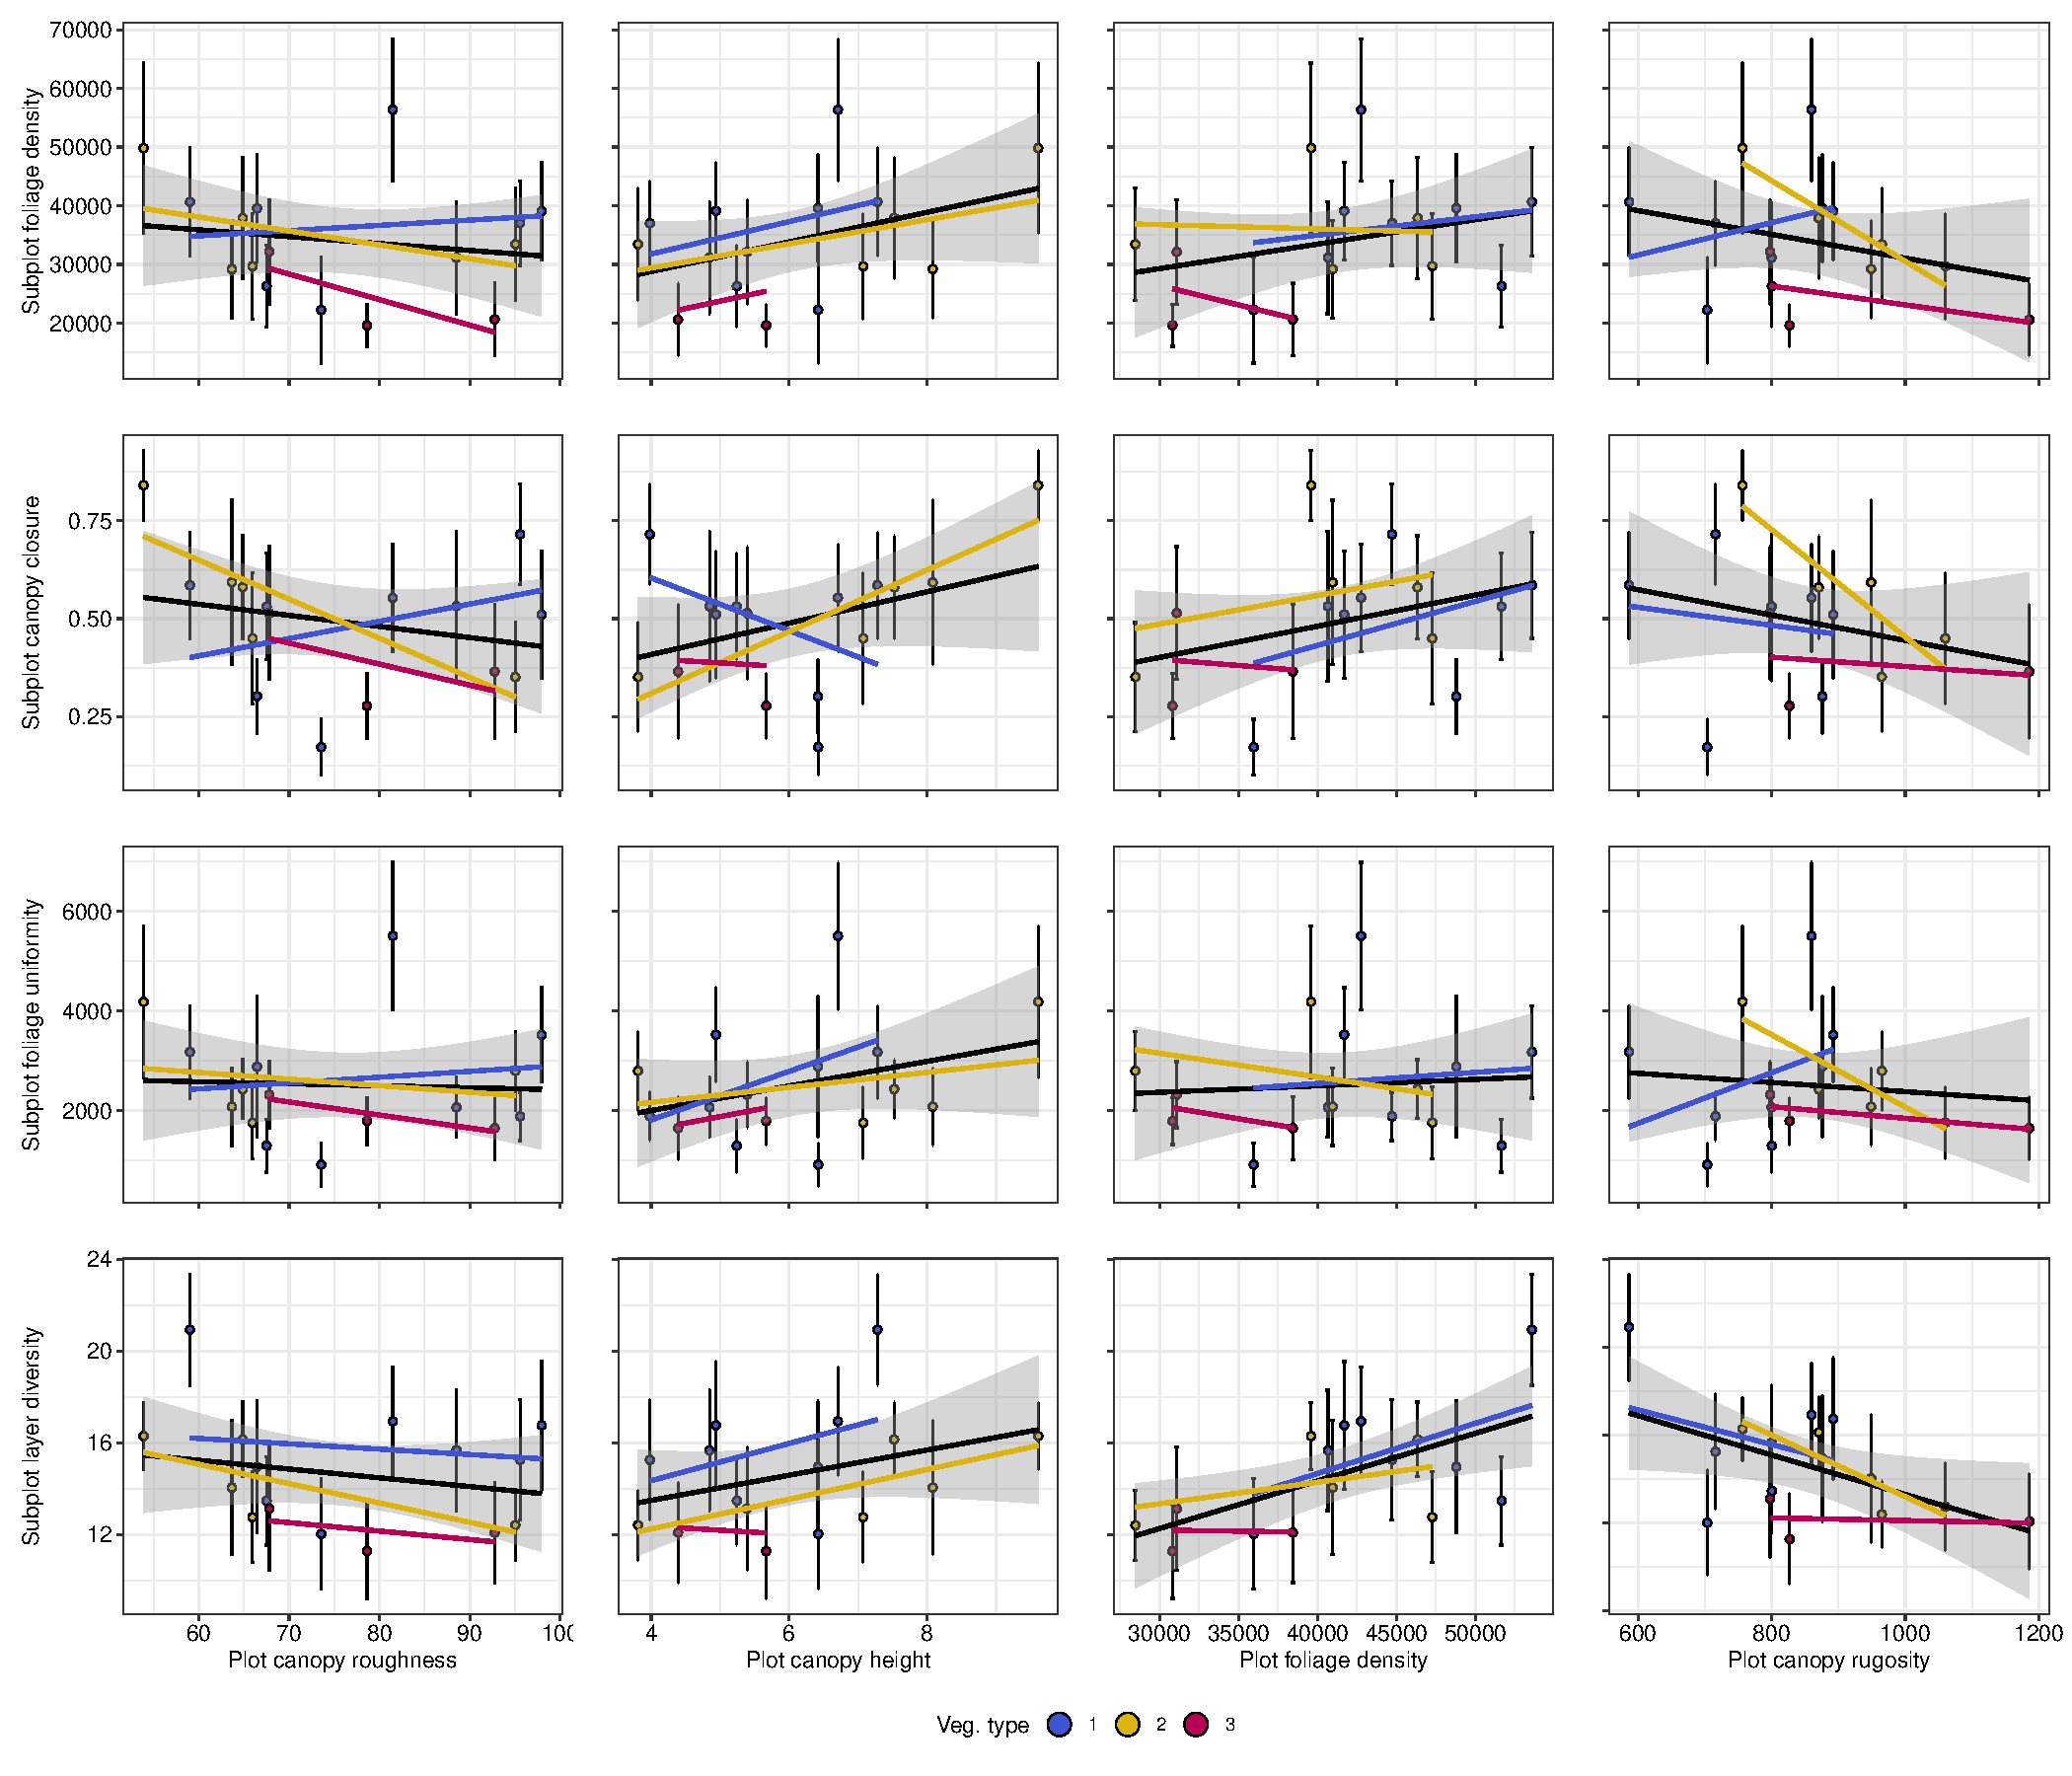
\includegraphics[width=\linewidth]{img/plot_subplot_bivar}
	\caption[Bivariate plots comparing plot and subplot canopy complexity metrics]{Bivariate plots comparing canopy structural metrics at the plot (x axis) and subplot scale (y axis). Each point represents the mean values of a single plot. Points and linear model fits are coloured according to vegetation type. The black linear model combines all vegetation types. Error bars on points are the standard deviation of mean subplot metrics across the plot. Note that because plot level canopy closure is calculated as the mean of subplot canopy closure, a comparison of subplot and plot canopy closure is not made in this figure.}
	\label{tls:plot_subplot_bivar}
\end{figure}

\section{Discussion}
\label{tls:sec:discussion}

% Recap
This study investigated relationships between tree species diversity, stand structure, and several metrics of tree canopy complexity using terrestrial LiDAR in southern African savannas, with a view to improving understanding of the biotic drivers of variation in canopy complexity and vegetation dynamics. Species diversity appeared to generally have weak positive effects on canopy complexity metrics related to canopy density at both the subplot and plot scales. While biodiversity effects were weak this is not unexpected, as environmental heterogeneity and landscape history lead to a great deal of stochasticity in canopy structure at small spatial scales, which could obscure biodiversity effects. Plots with greater species diversity produced taller tree canopies, with greater canopy closure and foliage density. Species diversity had negative effects on canopy surface roughness and canopy rugosity, canopy complexity metrics both related to the spatial heterogeneity of foliage distribution. The study did not however, find support for the hypothesis that increased heterogeneity in tree stem size is related to an increase in canopy complexity, and only partial support for the hypothesis that greater spatial clustering of stems is associated with increased canopy complexity. This study supports previous studies in forests which found a positive association between tree species diversity and canopy space-filling \citep{Seidel2013, Shirima2015b}.

\subsection{Ecological consequences of a species diversity effect on canopy complexity}
\label{tls:ssec:ecology}

% Ecological consequences of the effect of species diversity on canopy complexity
The result that species diversity increases metrics of canopy density suggests that diverse stands can more effectively close the tree canopy under a given set of environmental conditions. Of course, environmental conditions remain the largest determinant of canopy cover and were not incorporated here. There are climate thresholds which may prevent canopy closure even in diverse savannas \citep{Devine2017}. Increased canopy closure reduces light penetration to the ground \citep{Pilon2020}, reducing grass fuel load, and so could promote woody densification in diverse stands under atmospheric CO\textsubscript{2} enrichment. Similarly, the finding that species diversity is associated with an increase in foliage density and canopy height suggests that more diverse stands could more effectively upregulate productivity in response to atmospheric CO\textsubscript{2} fertilisation, and can maintain stands with greater woody biomass. Taller trees hold disproportionately higher biomass than shorter trees \citep{King1990}. In mesic savannas that are prone to disturbance by fire, increased growth rate and canopy height could increase the likelihood of trees escaping the ``fire trap'', and facilitate their growth to larger canopy trees \citep{Wakeling2011}. This finding concurs with many previous studies, which have found that species diversity leads to greater woody productivity in both forests and savannas \citep{Plas2019, Liang2016}. This study adds further information on the mechanisms underlying the species diversity effect on ecosystem function in savannas, that niche complementarity among species promotes greater canopy occupancy.

\subsection{Species diversity and variation in tree size}
\label{tls:ssec:diversity}

% Covariance of basal area CV and shannon diversity
Path analysis showed that indirect effects of species diversity on canopy complexity via tree stem size (basal area CV) were negligible, due to the lack of an effect of tree stem size on canopy complexity at both the subplot and plot scale. This finding suggests that the effects of species diversity on canopy complexity are not simply due to covariation with heterogeneity of tree stem size, which could also arise due to demographic effects, rather they are due to differences among species in their canopy dimensions and growth strategy. This strengthens support for the hypothesis that species diversity genuinely increases canopy complexity and canopy density, and is not merely an artefactual relationship. Previous studies in temperate and boreal forests have suggested that increasing tree stem size diversity through active management and thinning can offset productivity losses caused by reduced species diversity \citep{Levick2009}, but this study suggests that in southern African savannas at least, this is not the case. 

% Decoupling of tree size and foliage volume
The lack of a strong effect of tree size variation on canopy complexity suggests a partial decoupling of tree size and foliage volume. This finding highlights that there are likely species-specific differences in growth strategy which influence crown shape, and physiological limits on crown architecture that lead to species diversity effects on canopy packing that are separate from those driven by tree size \citep{Panzou2020}. Thus, structural diversity in crown architecture appears to be a key mechanism by which species diversity affects ecosystem function in these savannas. Seminal work in southern African woodlands described the wide variety of tree functional forms in southern African woodlands \citep{Solbrig1996}, with highly adaptive growth strategies to escape the ``fire-trap'' \citep{Dantas2013}. 

Shannon diversity did have strong positive effects on tree stem size variation and tree density. This can be interpreted as a niche complementarity effect, where diverse savannas are able to support a greater density of trees by reducing the effects of intraspecific competition and promoting canopy occupation in different vertical layers by trees of different sizes. Although basal area CV was included in best models for subplot layer diversity and foliage density, subplot level path analysis suggests that covariance between basal area CV and species diversity, and the effect of species diversity on canopy complexity, means that any observed effect of basal area CV on subplot canopy complexity is actually due to species diversity rather than covarying with basal area CV. 

% Tree density drops out of most of the plot mixed models. 
Despite tree density having strong positive observed effects on canopy density, and negative effects on canopy heterogeneity metrics in bivariate relationships, tree density only appeared in the best quality plot level mixed model for canopy rugosity. Additionally, the effect sizes for tree density in maximal mixed models were small. At the subplot level however, the Hegyi crowding index, which can be seen as analogous to tree density at neighbourhood scales, was a strong determinant of canopy complexity. Tree density was shown to covary with basal area CV and Voronoi cell area CV at the plot scale, which described variation in tree size and degree of spatial clustering, respectively. This covariance may have led to the effect dropping out in the best models at the plot scale, while at the subplot scale there were no measures of spatial clustering included. Hegyi crowding and tree density are expected to positively correlate with resource availability, and negatively correlate with disturbance which causes tree mortality and reduces tree growth. The study sites sampled here did cover a gradient of tree density, but variation in tree density within vegetation types was small. As vegetation type was included as a random effect in mixed models, this may have led to tree density not having a larger effect size in the models.

Variation in tree size was related to positive canopy complexity effects for within-canopy structural metrics such as layer diversity and canopy surface roughness, but had negligible effects on canopy density. This is in line with other studies in forest ecosystems, which report that variation in tree size increases total canopy volume occupancy by increasing the number of canopy layers, but does not necessarily result in a concomitant increase in canopy closure, as the resulting canopies are often more sparse, due to increased competition for light \citep{Beland2021a}. Both path analyses also support this conclusion, where species diversity was found to cause an increase in stand structural diversity, but this did not extend to an increase in canopy closure. 

\subsection{Spatial clustering effects}
\label{tls:ssec:clustering}

% Contrasting effects of spatial regularity and spatial clustering
Spatial regularity of stems, measured using the uniform angle index, was associated with a clear decrease in canopy closure, with similar behaviour across vegetation types. Uniform angle index was also included in the best multivariate model predicting canopy closure. Concurrently, spatial clustering of stems, measured by Voronoi cell area CV was included in the best model for foliage density but had a positive effect on this canopy complexity metric. This finding is expected, as spatial clustering results in reduced canopy cover in areas outside clusters, and a non-compensatory increase in canopy closure within clusters, due to competition among individuals \citep{Martens2000}. In contrast, changes in spatial regularity of trees do not imply changes in the distance of stems, only their relative angular positions, though this does generally correlate with spatial clustering \citep{Gadow2002}.

Spatial mingling of species at the plot level had a moderately strong negative effect on canopy height. Mingling also had a negative effect on tree density and on tree size variation, and a positive effect on canopy surface roughness. These results are in line with initial expectations that conspecific clustering reduces canopy complexity and thus foliage volume, by increasing competition among nearby conspecific individuals. Spatial mingling was lowest in the \textit{Baikiaea} woodlands in Cluster 3, which also are expected to experience the most frequent and intense disturbance by fire of the vegetation types studied here, as a result of their sparse canopy and prolific grass growth on sandy well-drained soils (\autoref{intro:baikiaea}, \autoref{tls:veg_type_tile}). Together, these findings suggest that conspecific clustering is increased in the most disturbed plots, where clustering is promoted by a positive feedback where clustered individuals create protection from fire by reducing grass growth and forming thickets \citep{CharlesDominique2018}. Additionally, fire-adapted species frequently reproduce by suckering \citep{Hoffmann1998}, creating a positive density dependence effect whereby neighbouring trees are more likely to be of the same species. Spatial mingling is therefore probably a result of fire disturbance, which in turn correlates with other canopy complexity and structural metrics also affected by disturbance.

\subsection{Plot vs. subplot scale results}
\label{tls:ssec:plot_subplot}

% Plot level more clear than subplot level
The standardised effect sizes of species diversity on canopy complexity metrics were generally greater at the plot level than at the subplot level. While positive and significant relationships between species diversity and subplot canopy complexity metrics were observed in the subplot bivariate models, subplot linear mixed effects models did not show strong species diversity effects, and models were instead dominated by the effect of crowding. This finding suggests a large degree of stochastic variability in canopy complexity within plots, that can mask species effects at smaller spatial scales. The prevalence of disturbance events such as fire and damage by elephants in southern African woodlands \citep{Bond2008}, as well as tree-fall, small-scale variability in edaphic factors, and stochastic tree mortality all contribute to heterogeneity in canopy complexity \citep{Shirima2015b}. While disturbances are controlled to some extent by stand structure and composition, due to the stochastic nature of disturbance events, a snapshot study such as this cannot capture the average disturbance regime and there is therefore a great deal of noise in models predicting canopy complexity from species diversity. The contrast in strength of species diversity effects at the subplot and plot level demonstrates the importance of large sample units, a high degree of spatial replication, and ideally a longer time scale when measuring canopy complexity, especially in disturbed systems, to effectively account for inherent heterogeneity in the system. Even with the one hectare plots used in this study, these plots may still be too small to fully capture larger scale patch dynamics arising from disturbance feedbacks and edaphic heterogeneity.

\subsection{Variation among vegetation types}
\label{tls:ssec:veg_type_var}

% Variation among vegetation types
Bivariate relationships showed that some of the observed species diversity effect on canopy closure and foliage density may be driven by vegetation type, and the variation in species diversity among vegetation types. The linear mixed model framework however, which accounted for differences among vegetation types, still shows weak species diversity effects even after vegetation type is controlled for, strengthening the validity of the result. Canopy complexity metrics also differed among vegetation types, but significant differences among vegetation types only occurred in a few cases, mostly between miombo and non-miombo vegetation clusters. Canopy density and total foliage volume was lowest in ex-Acacia plots, as expected, while the highest canopy density occurred in miombo plots in Clusters 1 and 2. Miombo woodlands frequently have contiguous canopies with overlapping individual tree canopies \citep{Solbrig1996}, while ex-Acacia savannas show greater negative density dependence of individuals, forming patchy canopies with simpler vertical profiles \citep{Pillay2012}. From this result it is suggested that under identical disturbance and climatic regimes, ex-Acacia savannas may not be as effective at closing their canopy to exclude grasses. Particularly, the lower maximum tree height of trees in the ex-Acacia plots may preclude these savannas from forming a multi-layer canopy that may be necessary to allow increased biomass.

While vegetation types differed in mean values for stand structural and species diversity metrics, variation in these metrics produced results of similar direction and magnitude among vegetation types in most cases where strong effects were observed, suggesting that ecosystem processes driving canopy complexity are similar, even across these varied savanna types. Small sample sizes for \textit{Baikiaea} and ex-Acacia vegetation however, led to wide errors on most relationships, especially at the plot level, such that it is impossible to draw deep conclusions about the behaviour of these vegetation types. Variation in mean values of canopy complexity metrics among vegetation types is likely driven by species identity and variation in physiological limits on tree physiognomy \citep{Seidel2013, Sercu2017}, though species composition itself is driven by environmental factors and disturbance regime \citep{Ribeiro2020}. 

\section{Conclusion}
\label{tls:sec:conclusion}

Here I explored how tree species diversity and stand structure influence canopy complexity in southern African savannas, using terrestrial LiDAR methods. I determined that species diversity was related an increase in canopy metrics related to foliage density, and was independently related to variation in tree size and tree density. Together these results suggest that diverse savannas may be able to upregulate their productivity and more effectively exclude grasses under atmospheric CO\textsubscript{2} enrichment conditions. Miombo woodlands exhibited stronger diversity effects than ex-Acacia or \textit{Baikiaea} woodlands, but replication in these other woodland types prevents deeper conclusions on this matter. The findings presented here have a range of consequences for savanna land managers that wish to predict future vegetation dynamics, particularly related to woody encroachment. This study also highlights and compares a number of novel and easy to calculate metrics for estimating different aspects of canopy complexity using terrestrial LiDAR, and sets a precedent as one of the few initial studies using terrestrial LiDAR in mesic savanna landscapes worldwide.

\newpage{}
\FloatBarrier{}
\begingroup
\setstretch{1.0}
\printbibliography[heading=subbibintoc]
\endgroup

\section{Supplementary material}
\label{tls:sec:supp}
\begin{supplement}

	\begin{figure}[H]
	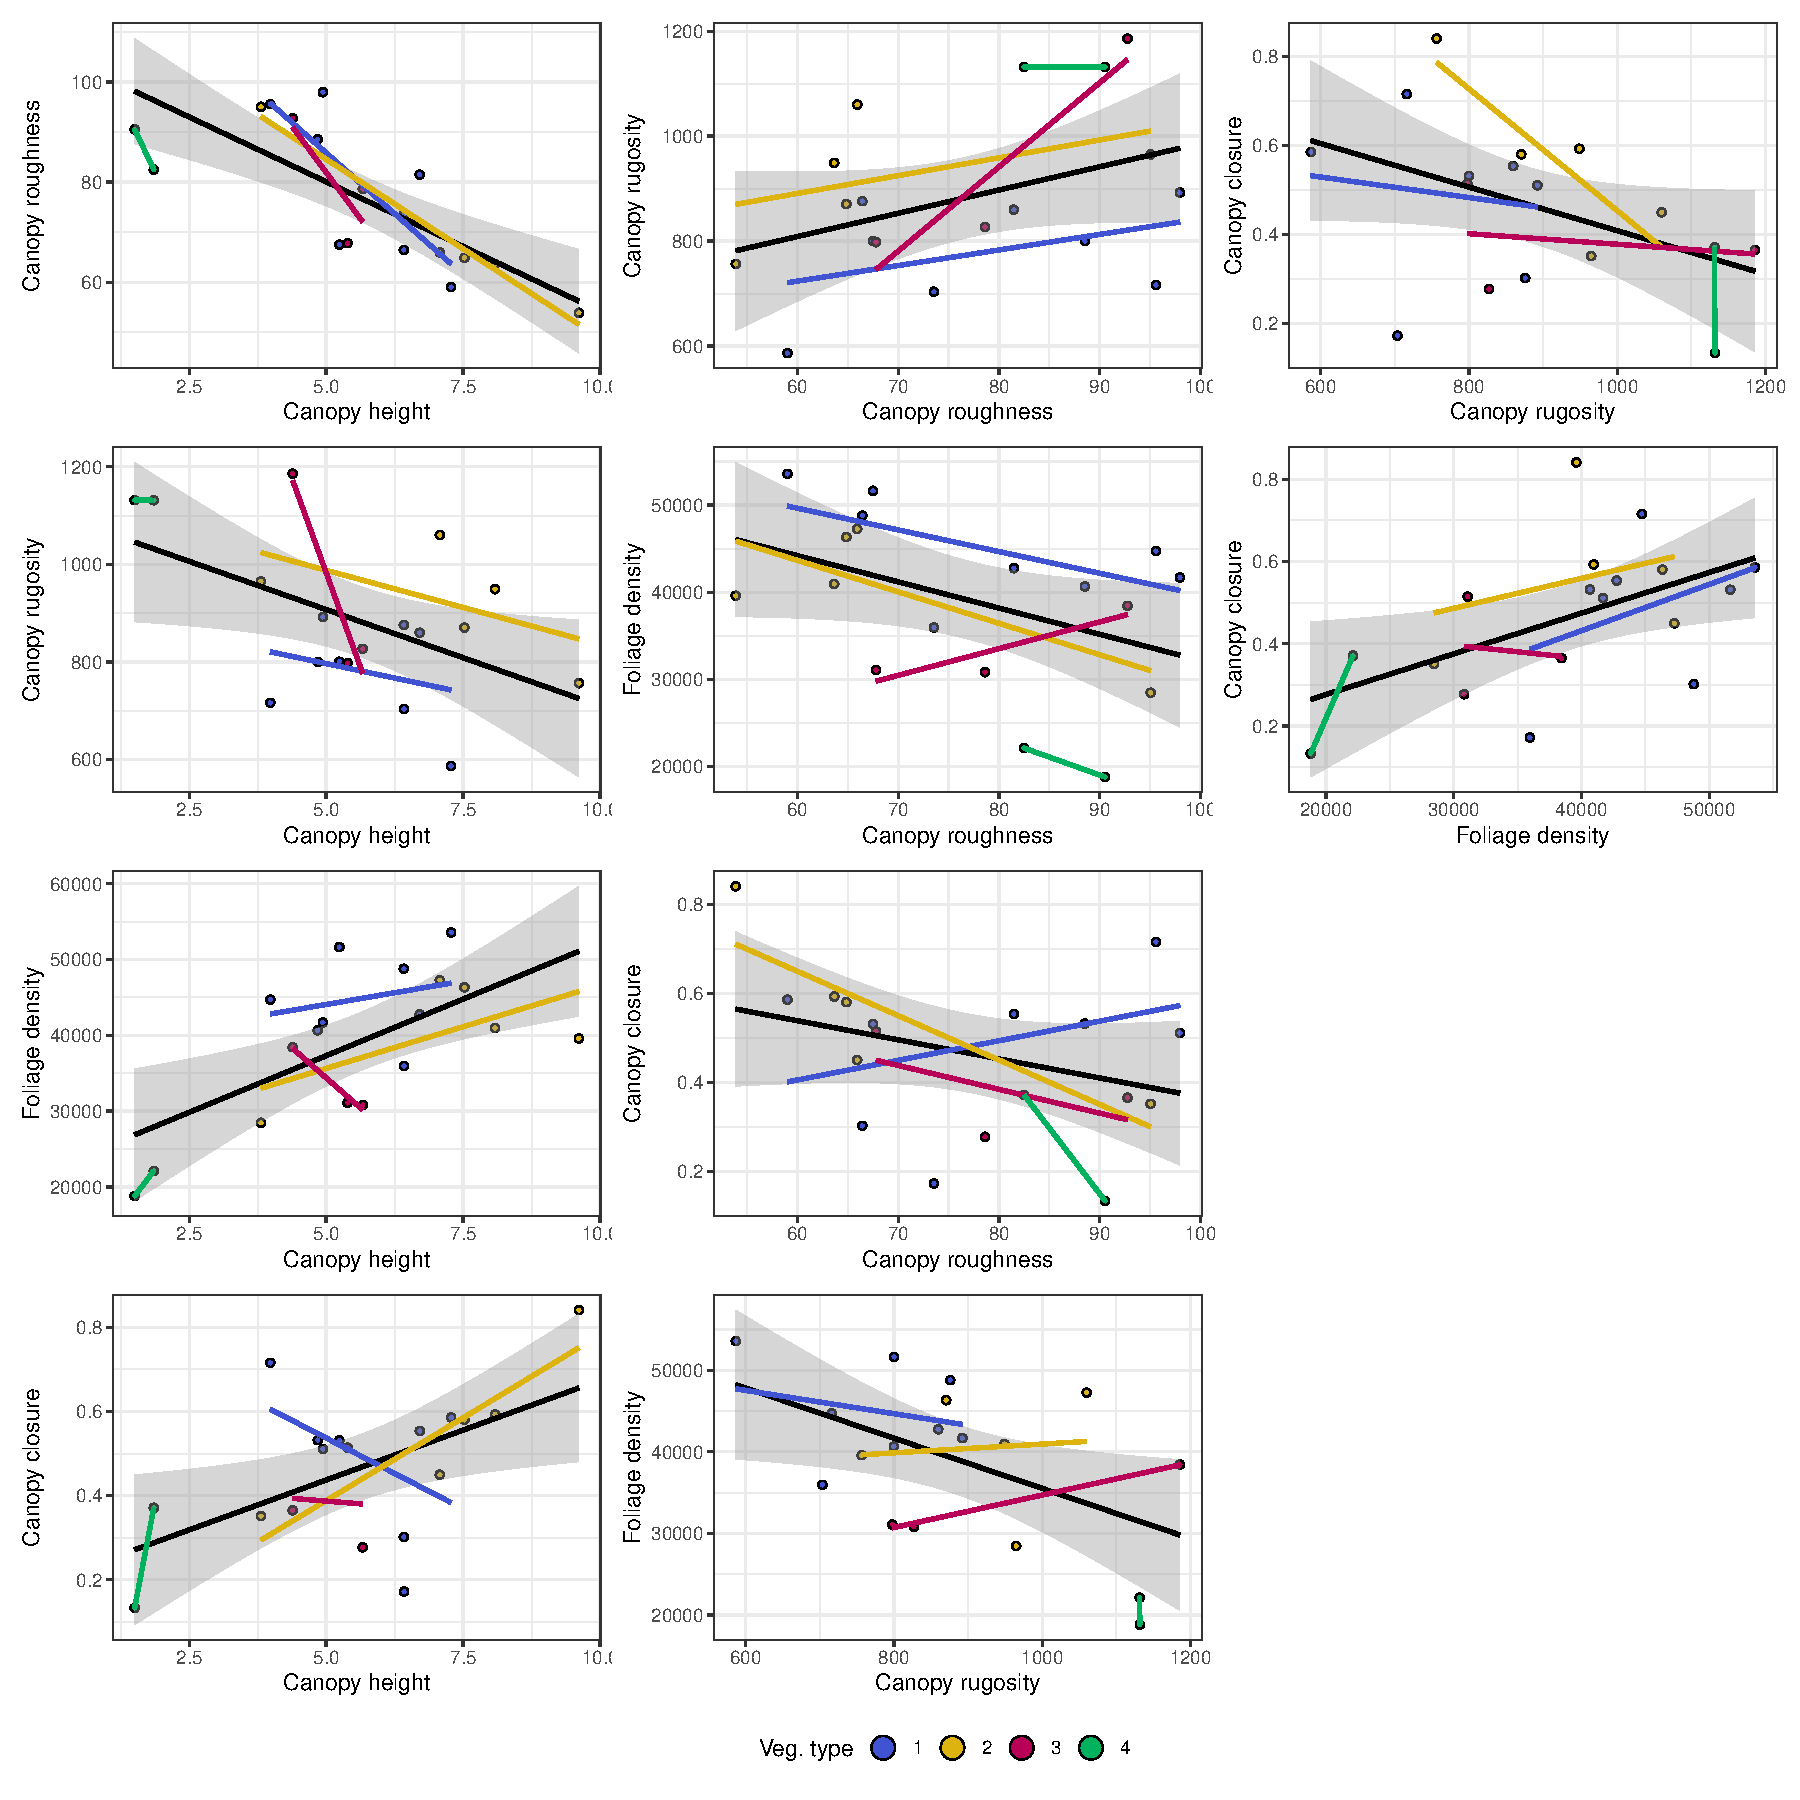
\includegraphics[width=\linewidth]{img/canopy_metric_comp_plot}
	\caption[Bivariate plots of plot canopy complexity metrics]{Bivariate scatter plots of plot level canopy complexity metrics.}
	\label{tls:canopy_metric_comp_plot}
\end{figure}

\begin{figure}[H]
	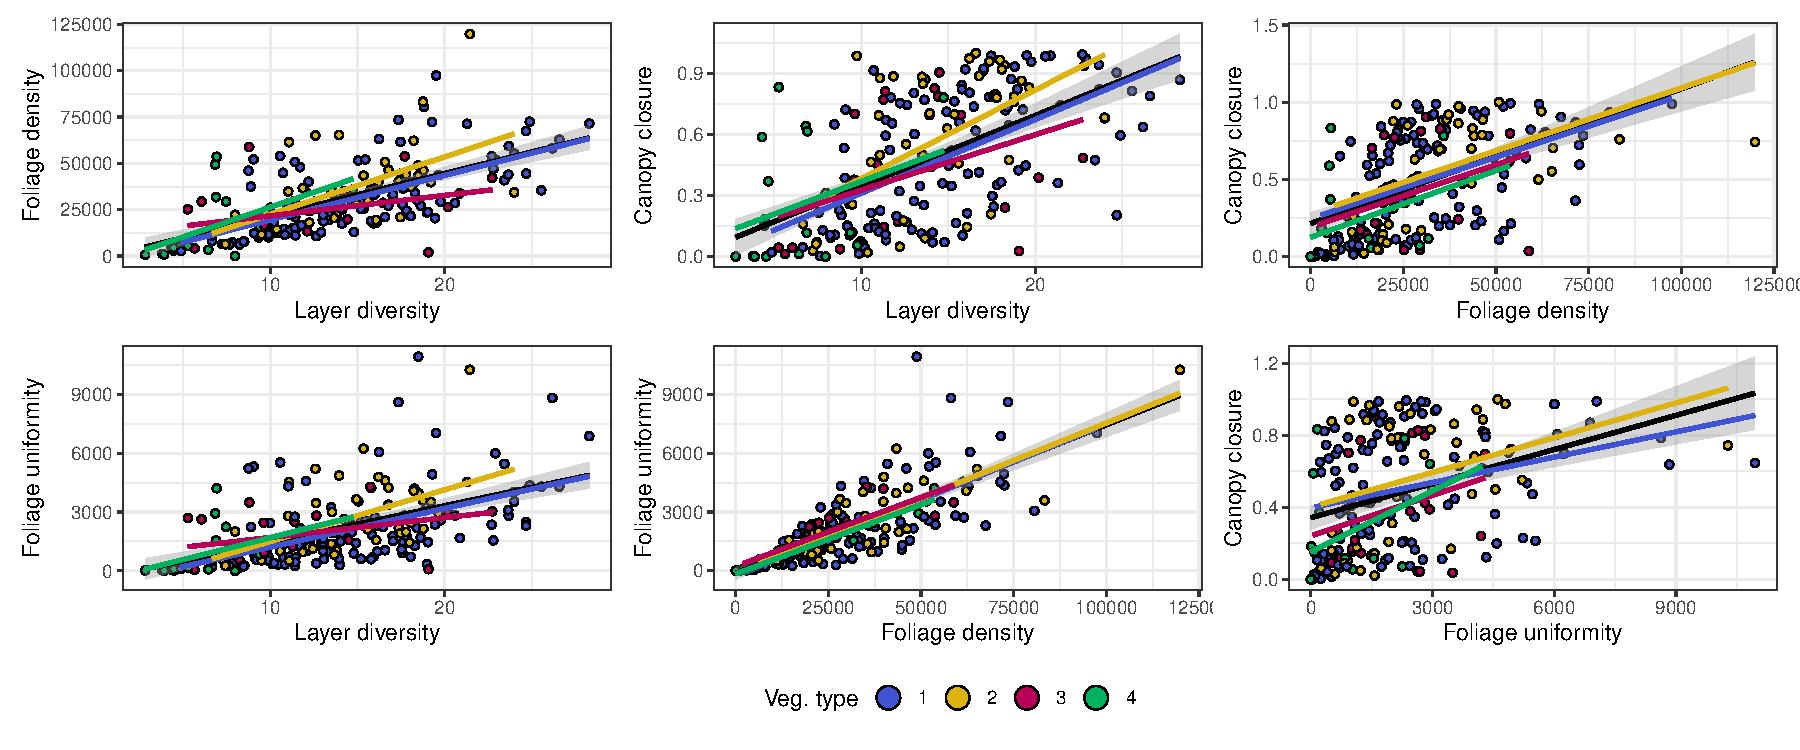
\includegraphics[width=\linewidth]{img/canopy_metric_comp_subplot}
	\caption[Bivariate plots of subplot canopy complexity metrics]{Bivariate scatter plots of subplot level canopy complexity metrics.}
	\label{tls:canopy_metric_comp_subplot}
\end{figure}

\begin{figure}[H]
	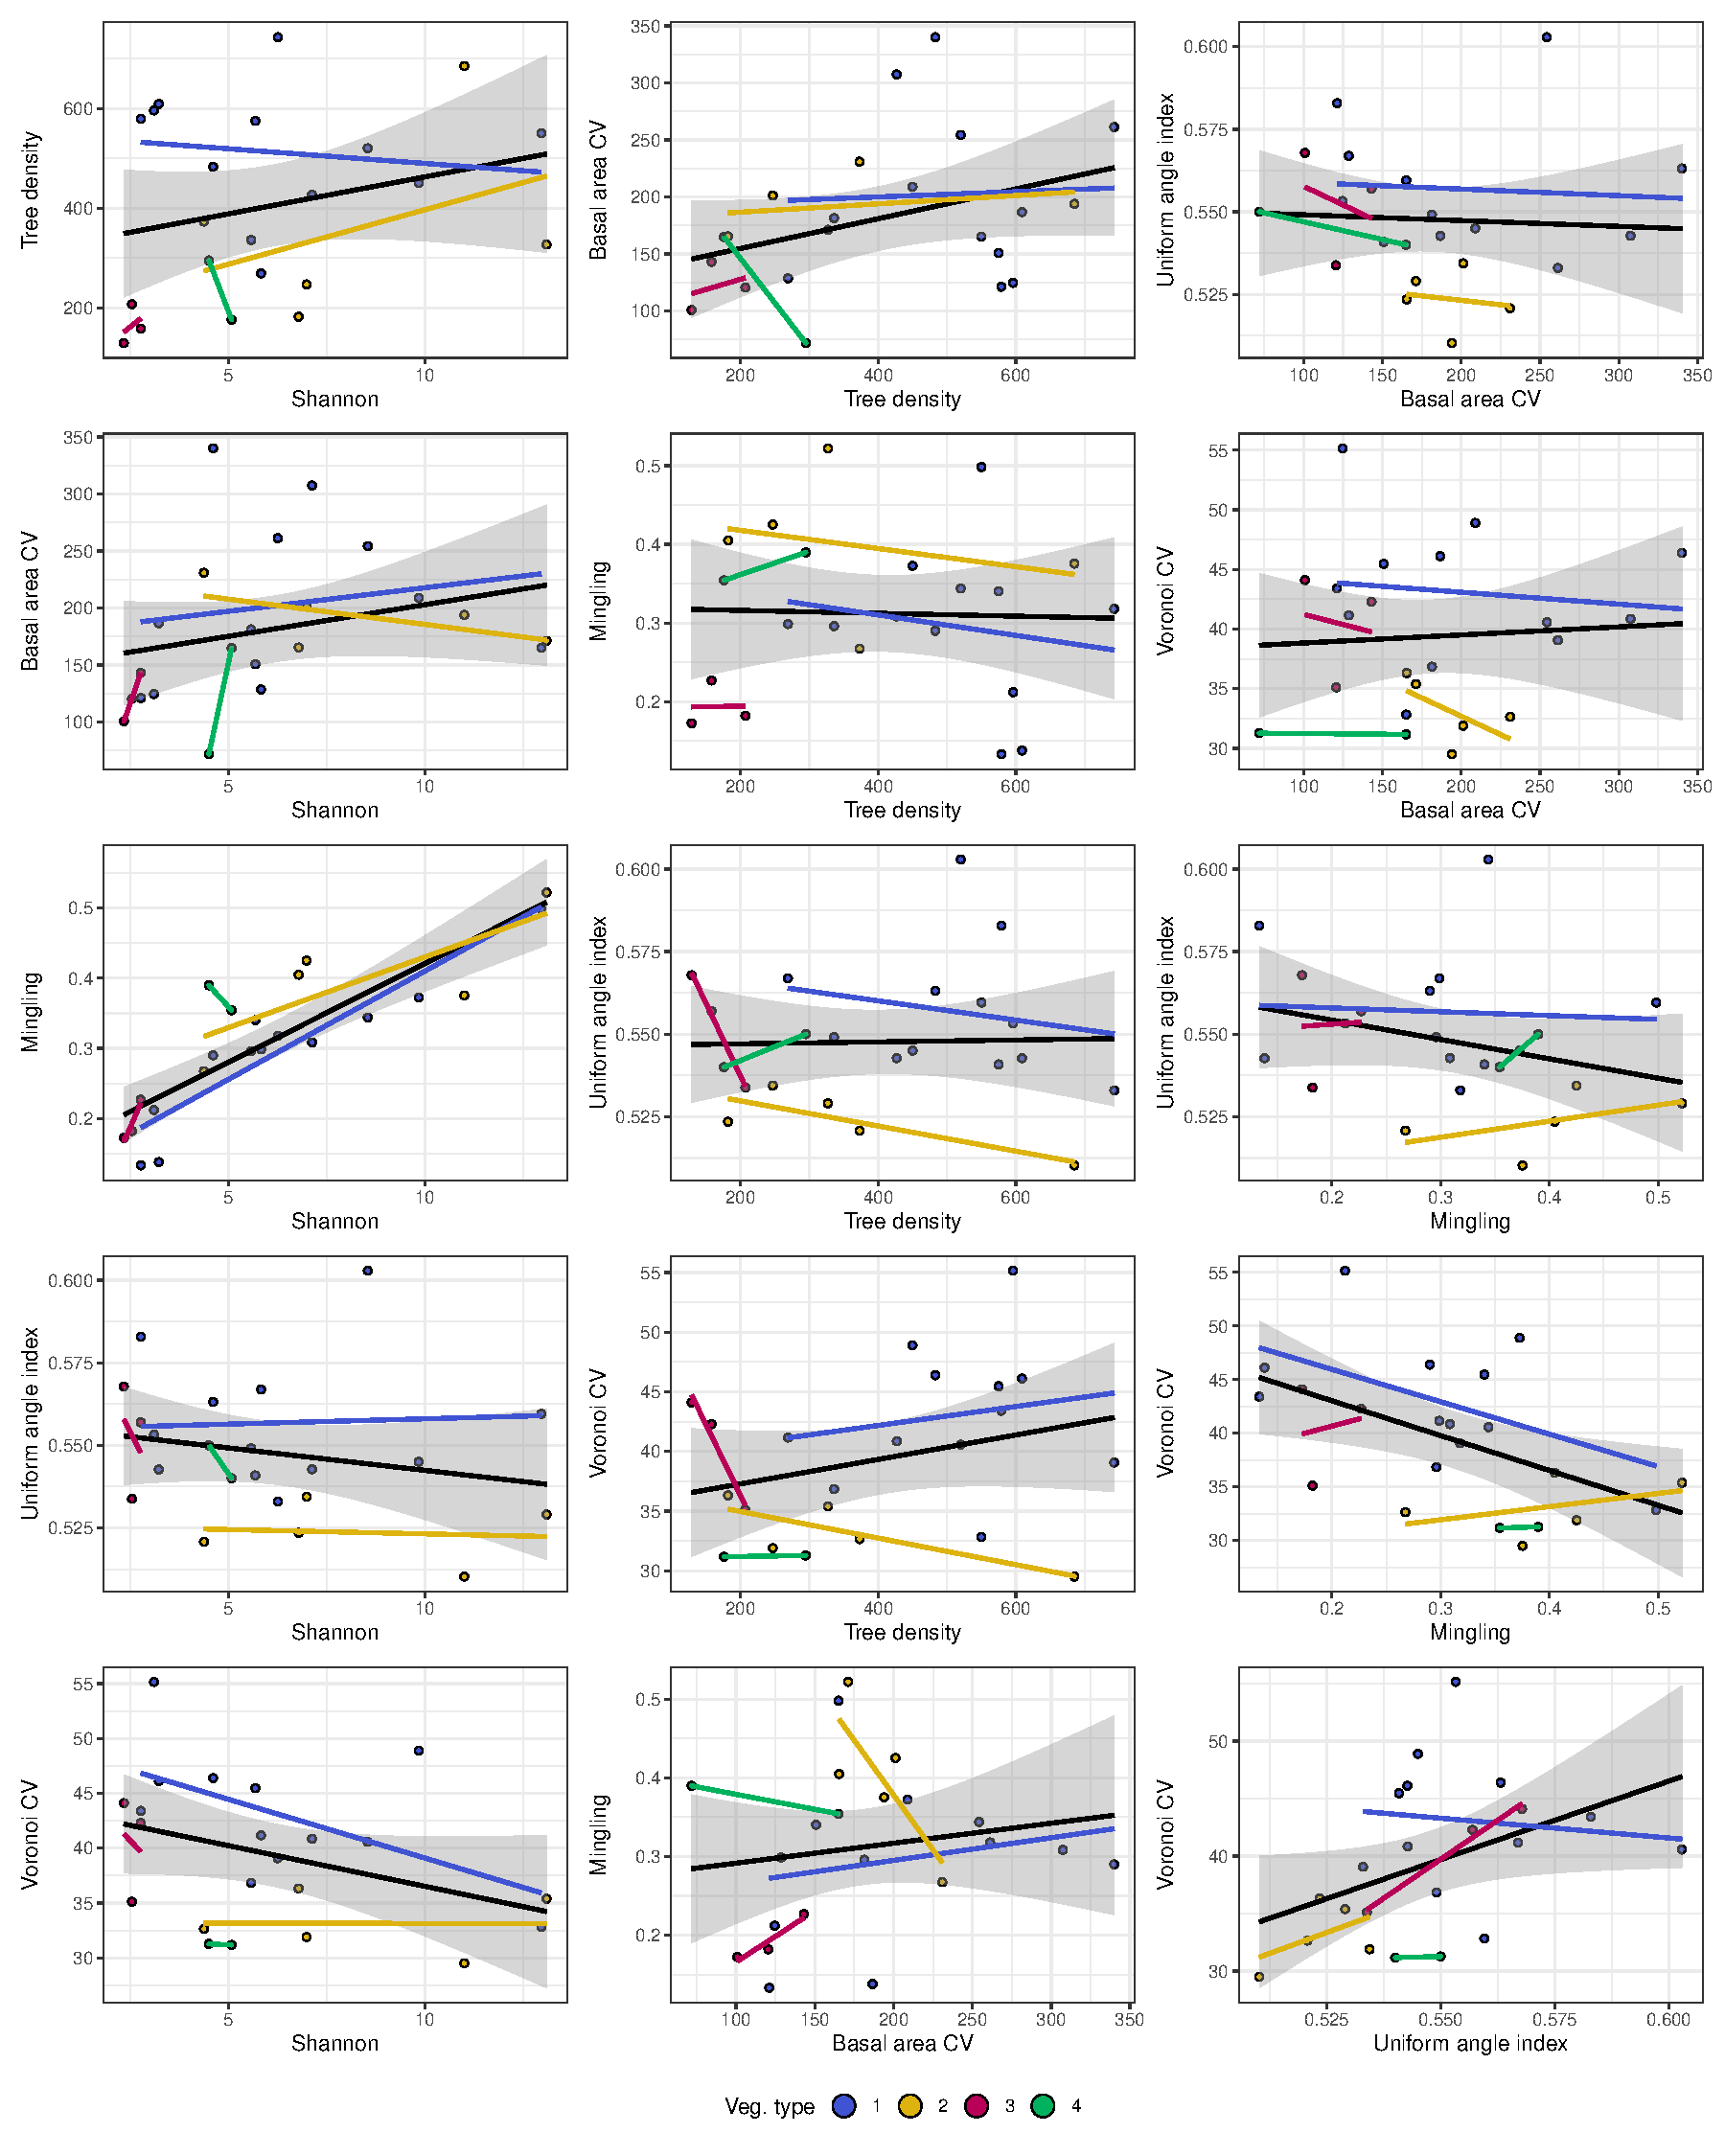
\includegraphics[width=\linewidth]{img/pred_comp_plot}
	\caption[Bivariate plots of plot diversity and stand structural metrics]{Bivariate scatter plots of plot level diversity and stand structural metrics.}
	\label{tls:pred_comp_plot}
\end{figure}

\begin{figure}[H]
	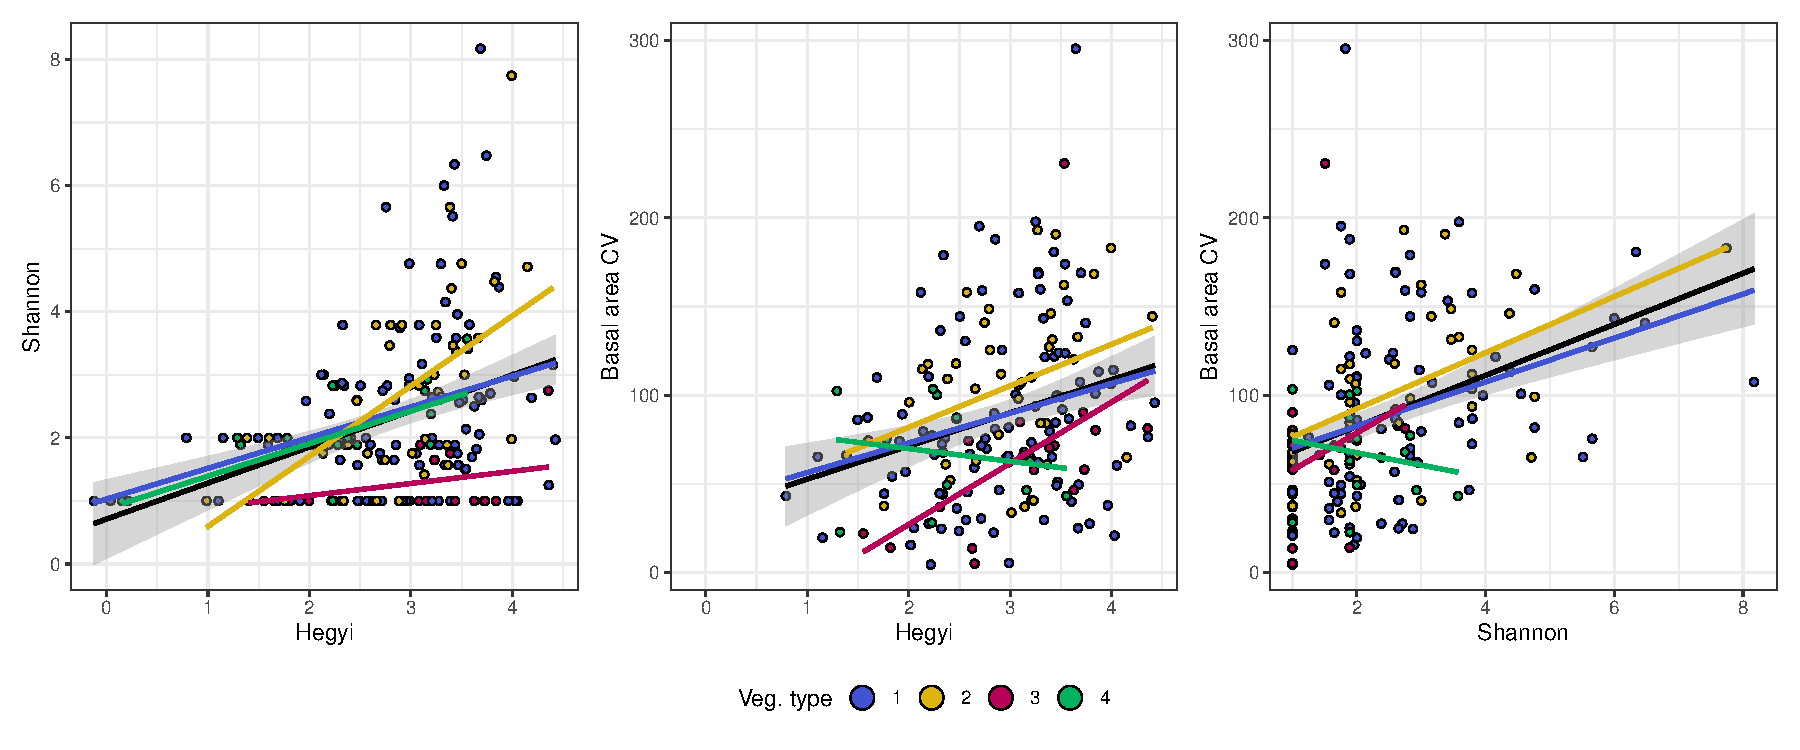
\includegraphics[width=\linewidth]{img/pred_comp_subplot}
	\caption[Bivariate plots of subplot diversity and stand structural metrics]{Bivariate scatter plots of subplot level diversity and stand structural metrics.}
	\label{tls:pred_comp_subplot}
\end{figure}


\begin{landscape}
	% latex table generated in R 4.1.0 by xtable 1.8-4 package
% Fri Aug 27 10:40:49 2021
\setlength{\tabcolsep}{4pt}
\begin{longtable}{llccccS[table-format=-2.2, table-space-text-post = {***}]}
\caption[Bivariate linear model summary by vegetation type]{Summary statistics of bivariate linear models comparing canopy complexity metrics with diversity and stand structural metrics, grouped by vegetation type. Note that models plot level canopy complexity metrics could not be fitted for Cluster 4, as this cluster only contained two plots. Slope refers to the slope of the predictor term in the model, $\pm$1 standard error.  T is the t-value of the slope of the predictor term in the model, Asterisks indicate the p-value of these terms (***<0.001, **<0.01, *<0.05).} \\ 
  \toprule
{Response} & {Predictor} & {Cluster} & {Slope} & {F} & {R\textsuperscript{2}} & {T} \\ 
  \midrule
\endfirsthead
\toprule
{Response} & {Predictor} & {Cluster} & {Slope} & {F} & {R\textsuperscript{2}} & {T} \\ 
\midrule
\endhead
{\multirow{4}{*}{Foliage density}} & {\multirow{4}{*}{Basal area CV}} & 1 &  7.3e+01$\pm$3.7e+01 & 4.0(2,97) & 0.04 & 1.99* \\*
   &  & 2 &  1.1e+02$\pm$7.9e+01 & 2.1(2,38) & 0.05 & 1.44 \\* 
   &  & 3 &  1.4e+01$\pm$7.2e+01 & 0.0(2,14) & 0.00 & 0.20 \\* 
   &  & 4 &  1.6e+01$\pm$2.0e+02 & 0.0(2,12) & 0.00 & 0.08 \\
   \midrule
{\multirow{4}{*}{Foliage density}} & {\multirow{4}{*}{Hegyi}} & 1 &  5.9e+03$\pm$2.1e+03 & 8.2(2,102) & 0.07 & 2.86** \\* 
   &  & 2 &  1.4e+04$\pm$3.6e+03 & 15.2(2,40) & 0.28 & 3.90*** \\* 
   &  & 3 &  6.6e+03$\pm$3.0e+03 & 4.8(2,23) & 0.17 & 2.18* \\* 
   &  & 4 &  1.5e+01$\pm$5.5e+03 & 0.0(2,13) & 0.00 & 0.00 \\ 
   \midrule
{\multirow{4}{*}{Foliage density}} & {\multirow{4}{*}{Shannon}} & 1 &  2.2e+03$\pm$1.3e+03 & 2.8(2,102) & 0.03 & 1.67 \\* 
   &  & 2 &  3.8e+03$\pm$2.4e+03 & 2.6(2,39) & 0.06 & 1.61 \\* 
   &  & 3 &  1.1e+04$\pm$6.5e+03 & 3.1(2,20) & 0.13 & 1.77 \\* 
   &  & 4 & -6.5e+03$\pm$6.5e+03 & 1.0(2,13) & 0.07 & -1.01 \\ 
   \midrule
{\multirow{4}{*}{Canopy closure}} & {\multirow{4}{*}{Basal area CV}} & 1 &  1.7e-04$\pm$6.0e-04 & 0.1(2,97) & 0.00 & 0.28 \\* 
   &  & 2 &  2.9e-03$\pm$1.1e-03 & 6.9(2,39) & 0.15 & 2.62* \\* 
   &  & 3 &  4.2e-03$\pm$1.1e-03 & 15.1(2,14) & 0.52 & 3.89** \\* 
   &  & 4 & -4.6e-03$\pm$3.0e-03 & 2.2(2,12) & 0.16 & -1.50 \\ 
   \midrule
{\multirow{4}{*}{Canopy closure}} & {\multirow{4}{*}{Hegyi}} & 1 &  2.2e-01$\pm$2.8e-02 & 62.3(2,102) & 0.38 & 7.89*** \\* 
   &  & 2 &  2.6e-01$\pm$5.1e-02 & 27.0(2,41) & 0.40 & 5.19*** \\* 
   &  & 3 &  2.8e-01$\pm$4.0e-02 & 50.7(2,23) & 0.69 & 7.12*** \\* 
   &  & 4 &  1.7e-01$\pm$8.0e-02 & 4.5(2,13) & 0.26 & 2.12 \\ 
   \midrule
{\multirow{4}{*}{Canopy closure}} & {\multirow{4}{*}{Shannon}} & 1 &  3.1e-03$\pm$2.2e-02 & 0.0(2,102) & 0.00 & 0.14 \\* 
   &  & 2 &  1.1e-01$\pm$3.2e-02 & 12.1(2,40) & 0.23 & 3.48** \\* 
   &  & 3 &  2.3e-01$\pm$1.4e-01 & 2.9(2,20) & 0.13 & 1.69 \\* 
   &  & 4 &  6.7e-02$\pm$1.1e-01 & 0.4(2,13) & 0.03 & 0.60 \\ 
   \midrule
{\multirow{4}{*}{Foliage uniformity}} & {\multirow{4}{*}{Basal area CV}} & 1 &  3.7e+00$\pm$4.0e+00 & 0.9(2,97) & 0.01 & 0.92 \\* 
   &  & 2 &  4.5e+00$\pm$7.4e+00 & 0.4(2,38) & 0.01 & 0.61 \\* 
   &  & 3 & -3.5e+00$\pm$5.9e+00 & 0.4(2,14) & 0.02 & -0.59 \\* 
   &  & 4 & -9.3e-01$\pm$1.5e+01 & 0.0(2,12) & 0.00 & -0.06 \\ 
   \midrule
{\multirow{4}{*}{Foliage uniformity}} & {\multirow{4}{*}{Hegyi}} & 1 &  2.2e+02$\pm$2.3e+02 & 1.0(2,102) & 0.01 & 0.98 \\* 
   &  & 2 &  7.5e+02$\pm$3.7e+02 & 4.0(2,40) & 0.09 & 2.00 \\* 
   &  & 3 &  4.5e+02$\pm$2.6e+02 & 2.9(2,23) & 0.11 & 1.72 \\* 
   &  & 4 & -7.5e+01$\pm$4.0e+02 & 0.0(2,13) & 0.00 & -0.19 \\ 
   \midrule
{\multirow{4}{*}{Foliage uniformity}} & {\multirow{4}{*}{Shannon}} & 1 &  2.3e+02$\pm$1.4e+02 & 2.6(2,102) & 0.02 & 1.61 \\* 
   &  & 2 &  8.6e+01$\pm$2.2e+02 & 0.1(2,39) & 0.00 & 0.38 \\* 
   &  & 3 &  1.3e+03$\pm$5.1e+02 & 6.1(2,20) & 0.23 & 2.48* \\* 
   &  & 4 & -5.9e+02$\pm$4.7e+02 & 1.6(2,13) & 0.11 & -1.27 \\ 
   \midrule
{\multirow{4}{*}{Layer diversity}} & {\multirow{4}{*}{Basal area CV}} & 1 &  2.5e-02$\pm$9.3e-03 & 7.1(2,97) & 0.07 & 2.66** \\* 
   &  & 2 &  3.9e-02$\pm$1.4e-02 & 8.0(2,38) & 0.17 & 2.83** \\* 
   &  & 3 &  2.7e-02$\pm$2.3e-02 & 1.3(2,14) & 0.09 & 1.15 \\* 
   &  & 4 &  2.1e-02$\pm$3.1e-02 & 0.5(2,12) & 0.04 & 0.67 \\ 
   \midrule
{\multirow{4}{*}{Layer diversity}} & {\multirow{4}{*}{Hegyi}} & 1 &  2.7e+00$\pm$4.9e-01 & 29.1(2,102) & 0.22 & 5.39*** \\* 
   &  & 2 &  2.0e+00$\pm$7.5e-01 & 7.1(2,40) & 0.15 & 2.66* \\* 
   &  & 3 &  1.9e+00$\pm$1.0e+00 & 3.6(2,23) & 0.13 & 1.89 \\* 
   &  & 4 &  1.1e+00$\pm$8.5e-01 & 1.8(2,13) & 0.12 & 1.33 \\ 
   \midrule
{\multirow{4}{*}{Layer diversity}} & {\multirow{4}{*}{Shannon}} & 1 &  1.0e+00$\pm$3.4e-01 & 8.7(2,102) & 0.08 & 2.95** \\* 
   &  & 2 &  9.5e-01$\pm$4.3e-01 & 4.8(2,39) & 0.11 & 2.18* \\* 
   &  & 3 &  4.9e+00$\pm$1.8e+00 & 7.2(2,20) & 0.26 & 2.68* \\* 
   &  & 4 &  1.8e-01$\pm$1.1e+00 & 0.0(2,13) & 0.00 & 0.16 \\ 
   \midrule
{\multirow{4}{*}{Canopy roughness}} & {\multirow{4}{*}{Basal area CV}} & 1 &  1.2e-01$\pm$6.9e-02 & 2.9(2,6) & 0.33 & 1.72 \\* 
   &  & 2 & -3.2e-01$\pm$2.9e-01 & 1.2(2,3) & 0.29 & -1.10 \\* 
   &  & 3 &  3.5e-01$\pm$4.7e-01 & 0.6(2,1) & 0.36 & 0.74 \\* 
   &  & 4 &  &  &  &  \\ 
   \midrule
{\multirow{4}{*}{Canopy roughness}} & {\multirow{4}{*}{Voronoi CV}} & 1 &  2.6e-01$\pm$1.2e+00 & 0.0(2,6) & 0.01 & 0.22 \\* 
   &  & 2 &  4.6e+00$\pm$1.9e+00 & 6.1(2,3) & 0.67 & 2.48 \\* 
   &  & 3 &  1.8e+00$\pm$1.9e+00 & 1.0(2,1) & 0.49 & 0.99 \\* 
   &  & 4 &  &  &  &  \\ 
   \midrule
{\multirow{4}{*}{Canopy roughness}} & {\multirow{4}{*}{Mingling}} & 1 & -4.2e+01$\pm$5.7e+01 & 0.5(2,6) & 0.08 & -0.74 \\* 
   &  & 2 &  1.6e+01$\pm$9.7e+01 & 0.0(2,3) & 0.01 & 0.17 \\* 
   &  & 3 &  3.5e+02$\pm$2.5e+02 & 2.0(2,1) & 0.67 & 1.42 \\* 
   &  & 4 &  &  &  &  \\ 
   \midrule
{\multirow{4}{*}{Canopy roughness}} & {\multirow{4}{*}{Tree density}} & 1 & -4.3e-02$\pm$4.5e-02 & 0.9(2,6) & 0.13 & -0.96 \\* 
   &  & 2 & -5.9e-02$\pm$3.1e-02 & 3.6(2,3) & 0.54 & -1.89 \\* 
   &  & 3 & -1.8e-01$\pm$2.6e-01 & 0.5(2,1) & 0.31 & -0.68 \\* 
   &  & 4 &  &  &  &  \\ 
   \midrule
{\multirow{4}{*}{Canopy roughness}} & {\multirow{4}{*}{Shannon}} & 1 & -2.3e+00$\pm$1.7e+00 & 1.7(2,6) & 0.22 & -1.32 \\* 
   &  & 2 & -1.4e+00$\pm$2.4e+00 & 0.4(2,3) & 0.11 & -0.60 \\* 
   &  & 3 &  3.4e+01$\pm$4.7e+01 & 0.5(2,1) & 0.34 & 0.72 \\* 
   &  & 4 &  &  &  &  \\ 
   \midrule
{\multirow{4}{*}{Canopy roughness}} & {\multirow{4}{*}{Uniform angle index}} & 1 & -7.4e+01$\pm$2.6e+02 & 0.1(2,6) & 0.01 & -0.28 \\* 
   &  & 2 &  4.1e+02$\pm$9.5e+02 & 0.2(2,3) & 0.06 & 0.43 \\* 
   &  & 3 &  4.4e+02$\pm$5.7e+02 & 0.6(2,1) & 0.37 & 0.76 \\* 
   &  & 4 &  &  &  &  \\ 
   \midrule
{\multirow{4}{*}{Canopy height}} & {\multirow{4}{*}{Basal area CV}} & 1 & -6.5e-03$\pm$6.1e-03 & 1.1(2,6) & 0.16 & -1.07 \\* 
   &  & 2 &  4.3e-02$\pm$4.0e-02 & 1.2(2,3) & 0.28 & 1.08 \\* 
   &  & 3 & -3.1e-02$\pm$8.7e-03 & 12.3(2,1) & 0.92 & -3.51 \\* 
   &  & 4 &  &  &  &  \\ 
   \midrule
{\multirow{4}{*}{Canopy height}} & {\multirow{4}{*}{Voronoi CV}} & 1 & -1.0e-01$\pm$8.6e-02 & 1.5(2,6) & 0.20 & -1.21 \\* 
   &  & 2 & -7.0e-01$\pm$2.0e-01 & 12.7(2,3) & 0.81 & -3.57* \\* 
   &  & 3 & -1.8e-02$\pm$1.4e-01 & 0.0(2,1) & 0.02 & -0.13 \\* 
   &  & 4 &  &  &  &  \\ 
   \midrule
{\multirow{4}{*}{Canopy height}} & {\multirow{4}{*}{Mingling}} & 1 &  6.8e+00$\pm$3.8e+00 & 3.2(2,6) & 0.34 & 1.78 \\* 
   &  & 2 & -3.3e+00$\pm$1.3e+01 & 0.1(2,3) & 0.02 & -0.25 \\* 
   &  & 3 & -2.3e+01$\pm$9.3e-01 & 619.2(2,1) & 1.00 & -24.88* \\* 
   &  & 4 &  &  &  &  \\ 
   \midrule
{\multirow{4}{*}{Canopy height}} & {\multirow{4}{*}{Tree density}} & 1 & -3.5e-04$\pm$3.8e-03 & 0.0(2,6) & 0.00 & -0.09 \\* 
   &  & 2 &  8.6e-03$\pm$4.0e-03 & 4.7(2,3) & 0.61 & 2.16 \\* 
   &  & 3 & -1.0e-03$\pm$1.7e-02 & 0.0(2,1) & 0.00 & -0.06 \\* 
   &  & 4 &  &  &  &  \\
   \midrule
{\multirow{4}{*}{Canopy height}} & {\multirow{4}{*}{Shannon}} & 1 &  2.8e-01$\pm$1.1e-01 & 7.1(2,6) & 0.54 & 2.66* \\* 
   &  & 2 &  1.7e-01$\pm$3.3e-01 & 0.3(2,3) & 0.08 & 0.52 \\* 
   &  & 3 & -3.0e+00$\pm$9.0e-01 & 11.1(2,1) & 0.92 & -3.32 \\* 
   &  & 4 &  &  &  &  \\
   \midrule
{\multirow{4}{*}{Canopy height}} & {\multirow{4}{*}{Uniform angle index}} & 1 &  1.0e+01$\pm$2.1e+01 & 0.2(2,6) & 0.04 & 0.49 \\* 
   &  & 2 & -7.2e+01$\pm$1.3e+02 & 0.3(2,3) & 0.09 & -0.56 \\* 
   &  & 3 &  6.0e-02$\pm$3.9e+01 & 0.0(2,1) & 0.00 & 0.00 \\* 
   &  & 4 &  &  &  &  \\
   \midrule
{\multirow{4}{*}{Canopy closure}} & {\multirow{4}{*}{Basal area CV}} & 1 &  3.6e-04$\pm$6.9e-04 & 0.3(2,10) & 0.03 & 0.53 \\* 
   &  & 2 &  3.5e-03$\pm$3.5e-03 & 1.0(2,3) & 0.24 & 0.98 \\* 
   &  & 3 &  1.9e-03$\pm$5.3e-03 & 0.1(2,1) & 0.11 & 0.35 \\* 
   &  & 4 &  &  &  &  \\
   \midrule
{\multirow{4}{*}{Canopy closure}} & {\multirow{4}{*}{Voronoi CV}} & 1 &  9.3e-03$\pm$8.2e-03 & 1.3(2,10) & 0.11 & 1.13 \\* 
   &  & 2 & -6.6e-02$\pm$7.9e-03 & 69.7(2,3) & 0.96 & -8.35** \\* 
   &  & 3 & -2.5e-02$\pm$4.6e-03 & 29.0(2,1) & 0.97 & -5.39 \\* 
   &  & 4 &  &  &  &  \\
   \midrule
{\multirow{4}{*}{Canopy closure}} & {\multirow{4}{*}{Mingling}} & 1 & -1.6e-01$\pm$5.1e-01 & 0.1(2,10) & 0.01 & -0.31 \\* 
   &  & 2 & -6.9e-01$\pm$1.1e+00 & 0.4(2,3) & 0.12 & -0.63 \\* 
   &  & 3 &  7.6e-02$\pm$4.1e+00 & 0.0(2,1) & 0.00 & 0.02 \\* 
   &  & 4 &  &  &  &  \\
   \midrule
{\multirow{4}{*}{Canopy closure}} & {\multirow{4}{*}{Tree density}} & 1 &  1.4e-04$\pm$4.0e-04 & 0.1(2,10) & 0.01 & 0.36 \\* 
   &  & 2 &  8.5e-04$\pm$2.4e-04 & 12.2(2,3) & 0.80 & 3.50* \\* 
   &  & 3 &  3.0e-03$\pm$4.3e-06 & 499683.9(2,1) & 1.00 & 706.88*** \\* 
   &  & 4 &  &  &  &  \\
   \midrule
{\multirow{4}{*}{Canopy closure}} & {\multirow{4}{*}{Shannon}} & 1 & -7.6e-03$\pm$1.7e-02 & 0.2(2,10) & 0.02 & -0.45 \\* 
   &  & 2 &  8.5e-03$\pm$3.0e-02 & 0.1(2,3) & 0.03 & 0.28 \\* 
   &  & 3 &  1.9e-01$\pm$5.2e-01 & 0.1(2,1) & 0.12 & 0.37 \\* 
   &  & 4 &  &  &  &  \\
   \midrule
{\multirow{4}{*}{Canopy closure}} & {\multirow{4}{*}{Uniform angle index}} & 1 & -3.9e+00$\pm$2.3e+00 & 2.9(2,10) & 0.23 & -1.71 \\* 
   &  & 2 & -1.2e+01$\pm$9.3e+00 & 1.7(2,3) & 0.36 & -1.30 \\* 
   &  & 3 & -6.9e+00$\pm$3.9e-01 & 306.2(2,1) & 1.00 & -17.50* \\* 
   &  & 4 &  &  &  &  \\
   \midrule
{\multirow{4}{*}{Foliage density}} & {\multirow{4}{*}{Basal area CV}} & 1 & -4.5e+01$\pm$2.9e+01 & 2.3(2,6) & 0.28 & -1.52 \\* 
   &  & 2 &  1.5e+02$\pm$1.4e+02 & 1.1(2,3) & 0.27 & 1.05 \\* 
   &  & 3 &  1.8e+02$\pm$8.9e+01 & 4.2(2,1) & 0.81 & 2.06 \\* 
   &  & 4 &  &  &  &  \\
   \midrule
{\multirow{4}{*}{Foliage density}} & {\multirow{4}{*}{Voronoi CV}} & 1 &  3.5e+01$\pm$5.0e+02 & 0.0(2,6) & 0.00 & 0.07 \\* 
   &  & 2 & -7.7e+02$\pm$1.5e+03 & 0.3(2,3) & 0.08 & -0.51 \\* 
   &  & 3 &  2.7e+02$\pm$8.7e+02 & 0.1(2,1) & 0.09 & 0.31 \\* 
   &  & 4 &  &  &  &  \\
   \midrule
{\multirow{4}{*}{Foliage density}} & {\multirow{4}{*}{Mingling}} & 1 &  4.5e+03$\pm$2.5e+04 & 0.0(2,6) & 0.01 & 0.18 \\* 
   &  & 2 &  8.0e+02$\pm$4.7e+04 & 0.0(2,3) & 0.00 & 0.02 \\* 
   &  & 3 &  1.5e+05$\pm$2.0e+04 & 54.1(2,1) & 0.98 & 7.35 \\* 
   &  & 4 &  &  &  &  \\
   \midrule
{\multirow{4}{*}{Foliage density}} & {\multirow{4}{*}{Tree density}} & 1 &  8.8e+00$\pm$2.0e+01 & 0.2(2,6) & 0.03 & 0.45 \\* 
   &  & 2 &  1.1e+01$\pm$2.1e+01 & 0.3(2,3) & 0.08 & 0.51 \\* 
   &  & 3 & -1.3e+01$\pm$1.1e+02 & 0.0(2,1) & 0.01 & -0.12 \\* 
   &  & 4 &  &  &  &  \\
   \midrule
{\multirow{4}{*}{Foliage density}} & {\multirow{4}{*}{Shannon}} & 1 &  2.5e+02$\pm$8.1e+02 & 0.1(2,6) & 0.02 & 0.31 \\* 
   &  & 2 &  5.0e+02$\pm$1.2e+03 & 0.2(2,3) & 0.05 & 0.42 \\* 
   &  & 3 &  1.8e+04$\pm$9.1e+03 & 3.9(2,1) & 0.80 & 1.98 \\* 
   &  & 4 &  &  &  &  \\
   \midrule
{\multirow{4}{*}{Foliage density}} & {\multirow{4}{*}{Uniform angle index}} & 1 & -1.1e+05$\pm$1.0e+05 & 1.3(2,6) & 0.18 & -1.15 \\* 
   &  & 2 &  1.2e+05$\pm$4.7e+05 & 0.1(2,3) & 0.02 & 0.25 \\* 
   &  & 3 &  4.3e+04$\pm$2.5e+05 & 0.0(2,1) & 0.03 & 0.18 \\* 
   &  & 4 &  &  &  &  \\
   \midrule
{\multirow{4}{*}{Canopy rugosity}} & {\multirow{4}{*}{Basal area CV}} & 1 & -1.0e-01$\pm$6.1e-01 & 0.0(2,6) & 0.00 & -0.17 \\* 
   &  & 2 & -2.2e+00$\pm$2.2e+00 & 1.1(2,3) & 0.26 & -1.03 \\* 
   &  & 3 &  8.7e+00$\pm$5.4e+00 & 2.6(2,1) & 0.73 & 1.62 \\* 
   &  & 4 &  &  &  &  \\
   \midrule
{\multirow{4}{*}{Canopy rugosity}} & {\multirow{4}{*}{Voronoi CV}} & 1 &  7.9e+00$\pm$8.2e+00 & 0.9(2,6) & 0.13 & 0.96 \\* 
   &  & 2 &  3.5e+01$\pm$1.3e+01 & 6.8(2,3) & 0.69 & 2.61 \\* 
   &  & 3 &  1.8e+01$\pm$4.2e+01 & 0.2(2,1) & 0.15 & 0.42 \\* 
   &  & 4 &  &  &  &  \\
   \midrule
{\multirow{4}{*}{Canopy rugosity}} & {\multirow{4}{*}{Mingling}} & 1 & -5.9e+02$\pm$3.6e+02 & 2.7(2,6) & 0.31 & -1.63 \\* 
   &  & 2 &  8.5e+02$\pm$5.2e+02 & 2.7(2,3) & 0.47 & 1.63 \\* 
   &  & 3 &  7.2e+03$\pm$1.7e+03 & 17.6(2,1) & 0.95 & 4.19 \\* 
   &  & 4 &  &  &  &  \\
   \midrule
{\multirow{4}{*}{Canopy rugosity}} & {\multirow{4}{*}{Tree density}} & 1 & -1.9e-01$\pm$3.4e-01 & 0.3(2,6) & 0.05 & -0.56 \\* 
   &  & 2 & -4.6e-01$\pm$2.1e-01 & 4.9(2,3) & 0.62 & -2.22 \\* 
   &  & 3 & -1.2e+00$\pm$5.4e+00 & 0.0(2,1) & 0.05 & -0.22 \\* 
   &  & 4 &  &  &  &  \\
   \midrule
{\multirow{4}{*}{Canopy rugosity}} & {\multirow{4}{*}{Shannon}} & 1 & -2.4e+01$\pm$1.0e+01 & 5.3(2,6) & 0.47 & -2.31 \\* 
   &  & 2 &  6.4e+00$\pm$1.8e+01 & 0.1(2,3) & 0.04 & 0.35 \\* 
   &  & 3 &  8.5e+02$\pm$5.4e+02 & 2.5(2,1) & 0.71 & 1.57 \\* 
   &  & 4 &  &  &  &  \\
   \midrule
{\multirow{4}{*}{Canopy rugosity}} & {\multirow{4}{*}{Uniform angle index}} & 1 & -2.6e+03$\pm$1.6e+03 & 2.5(2,6) & 0.30 & -1.58 \\* 
   &  & 2 &  1.0e+04$\pm$4.1e+03 & 6.1(2,3) & 0.67 & 2.47 \\* 
   &  & 3 &  3.4e+03$\pm$1.2e+04 & 0.1(2,1) & 0.07 & 0.28 \\* 
   &  & 4 &  &  &  &  \\
   \bottomrule
\label{tls:bivar_lm_summ_veg_type}
\end{longtable}


\end{landscape}

\end{supplement}

\end{refsection}

